% !TEX program = pdflatex
% ============================================================================
% Uzbekistan's Power Sector to 2040  --  two-column capstone research paper.
% Typeset by scripts/build_paper_latex.py from docs/Capstone_Report.md.
% Compiles with pdfLaTeX (Overleaf: default TeX Live). Run twice for the ToC.
% Figures live in ./figures/ (12 regenerated 300-DPI navy-palette PNGs).
% Author fills the amber [CITE]/[VERIFY]/[TEMPLATE] markers from her library.
% ============================================================================
\documentclass[10pt,twocolumn]{article}

\usepackage[T1]{fontenc}
\usepackage[utf8]{inputenc}     % source is ASCII after escaping; harmless to keep
\usepackage[default]{lato}      % humanist sans (DNV idiom) for body + headings
\usepackage[english]{babel}

% Horizontal margins held at 0.85in (column width unchanged -> no text reflow);
% vertical margins tightened to 0.72in to add ~0.26in of body height per page,
% which both fits more lines and gives the full-width floats more room to settle
% -- the deterministic lever for the <=30-page budget after Step-4 additions.
\usepackage[letterpaper,top=0.72in,bottom=0.72in,left=0.85in,right=0.85in,%
            headheight=13pt,headsep=9pt,columnsep=0.28in]{geometry}
\usepackage{graphicx}
\usepackage{booktabs}
\usepackage{array}
\usepackage{tabularx}
\newcolumntype{L}{>{\raggedright\arraybackslash}X}  % wrapping, left-ragged
\usepackage{amsmath}
\usepackage{amssymb}
\usepackage{siunitx}
\usepackage{textcomp}
\usepackage{xcolor}
\usepackage{caption}
\usepackage{titlesec}
\usepackage{titletoc}
\usepackage{enumitem}
\usepackage{fancyhdr}
\usepackage{lastpage}
\usepackage[most]{tcolorbox}     % DNV-style tinted key-finding callout panels
\usepackage[hidelinks]{hyperref}
\usepackage{xurl}                 % break long reference-list URLs anywhere (no overfull lines)

% ── DNV-style brand palette (matches figure_style_for_notebooks.py) ──────────
\definecolor{navy}{HTML}{003591}     % primary   — headings, rules, links
\definecolor{sky}{HTML}{9DC3E6}      % secondary — tinted callout/opener panels
\definecolor{skydeep}{HTML}{3E7CB1}  % legible mid-sky for rules on white
\definecolor{leaf}{HTML}{5C9A3C}     % accent/"good"
\definecolor{warmgrey}{HTML}{B4ADA3} % neutral
\definecolor{teal}{HTML}{3E7CB1}     % back-compat alias → mid-sky
\definecolor{amber}{HTML}{A85B00}    % action markers ONLY — deliberately unchanged
\definecolor{ink}{HTML}{1F2937}
\definecolor{rulegrey}{HTML}{B4ADA3}
\definecolor{metagrey}{HTML}{6B7280}   % calm grey for "reference complete" tags
\definecolor{panelgrey}{HTML}{EEF2F6} % very-pale panel tint for opener bands

\hypersetup{
  colorlinks=true, linkcolor=navy, urlcolor=navy, citecolor=navy,
  pdftitle={Uzbekistan's Power Sector to 2040},
  pdfauthor={Farangiz Jurakhonova}
}

% ── visible-but-distinct markers ─────────────────────────────────────────────
%   \mk      amber, action-needed: [CITE: ...] slots, [VERIFY: ...], [TEMPLATE]
%   \mkdone  calm grey, informational: [CITE-COMPLETE] (reference already filled)
\newcommand{\mk}[1]{{\color{amber}\small #1}}
\newcommand{\mkdone}[1]{{\color{metagrey}\footnotesize #1}}

% ── DNV-style key-finding callout ────────────────────────────────────────────
%   A pale-navy panel with a thick navy left bar carrying one headline number.
%   These quote figures already in the prose (no new quantity); they are a
%   design device that lifts the four results the brief flags as the stakes of
%   the report. \keystat{kicker}{big stat}{one-line gloss}.
\newtcolorbox{keystatbox}{
  enhanced, breakable=false, sharp corners,
  colback=panelgrey, colframe=panelgrey,
  borderline west={2.6pt}{0pt}{navy},
  boxrule=0pt, left=10pt, right=8pt, top=6pt, bottom=6pt,
  before skip=8pt, after skip=8pt,
}
\newcommand{\keystat}[3]{%
  \begin{keystatbox}%
  {\footnotesize\bfseries\color{skydeep}#1}\par\vspace{1pt}%
  {\Large\bfseries\color{navy}#2}\par\vspace{2pt}%
  {\footnotesize\color{ink}#3}%
  \end{keystatbox}}

% ── navy section headings, author's own numbering kept (unnumbered) ──────────
%   DNV chapter-opener idiom: the chapter (\section) head is set large in navy
%   with a thin sky rule drawn beneath it; subsections stay compact. The rule is
%   column-wide in the two-column body and page-wide on the front matter.
\titleformat{\section}{\normalfont\Large\bfseries\color{navy}}{}{0pt}{}
  [{\vspace{1pt}{\color{skydeep}\titlerule[1.1pt]}}]
\titleformat{\subsection}{\normalfont\normalsize\bfseries\color{navy}}{}{0pt}{}
\titlespacing*{\section}{0pt}{10pt}{5pt}
\titlespacing*{\subsection}{0pt}{6pt}{3pt}

% ── caption style: small, author's "Figure 2.1." text carries the number ─────
\captionsetup{font={small},labelformat=empty,justification=justified,
  singlelinecheck=false,skip=4pt}

% ── float placement: this is a float-heavy two-column paper (12 figures, 8
%    tables, most spanning both columns). Relax the default placement budget so
%    the starred (full-width) floats settle at page tops / float pages instead
%    of deferring and triggering "Too many unprocessed floats". Package-free. ──
\setcounter{topnumber}{3}\setcounter{dbltopnumber}{4}
\setcounter{bottomnumber}{2}\setcounter{totalnumber}{6}
\renewcommand{\topfraction}{0.92}\renewcommand{\dbltopfraction}{0.92}
\renewcommand{\bottomfraction}{0.5}\renewcommand{\textfraction}{0.08}
% \dblfloatpagefraction is the dominant lever for the "gap between graphs"
% complaint. At the old 0.66 a pair of medium figures (~75% of the page) was
% allowed to form a half-empty FLOAT PAGE, and the kernel's double-float page
% glue then spreads them apart with infinite stretch that \@fpsep/\raggedbottom
% cannot reach. Raising it to 0.88 forbids a float page unless the floats nearly
% fill it, so such pairs are instead set at the TOP of ordinary text pages (one
% per page top, body text beneath, \raggedbottom pooling any slack at the foot) —
% no mid-page gap. A genuinely page-filling figure still gets its own float page,
% where >88% occupancy leaves too little slack to spread visibly.
\renewcommand{\floatpagefraction}{0.85}\renewcommand{\dblfloatpagefraction}{0.88}
% Float-page vertical spacing. Pin floats to the TOP (\@fptop=0pt, no top
% stretch); give STACKED floats a fixed separation (\@fpsep) with no infinite
% "fil" — the default \@fpsep carries 2fil of stretch, and that is exactly what
% was injecting large blank gaps BETWEEN the graphs on figure-only pages; and
% let all leftover space pool at the BOTTOM (\@fpbot). Net effect: graphs stack
% snugly under one another at the top and the empty space sits below them.
\makeatletter
\setlength{\@fptop}{0pt}
\setlength{\@fpsep}{14pt plus 0pt minus 3pt}
\setlength{\@fpbot}{0pt plus 1fil}
\makeatother

% ── tighter float moats (DNV idiom is densely set) — reclaims the page the
%    Step-4 callouts/openers added without reshuffling float placement. The
%    \dbltextfloatsep governs the gap around the many full-width figure* / table*
%    floats and is the dominant lever here. ────────────────────────────────────
\setlength{\textfloatsep}{12pt plus 2pt minus 2pt}
\setlength{\dbltextfloatsep}{12pt plus 2pt minus 2pt}
\setlength{\floatsep}{9pt plus 2pt minus 2pt}
\setlength{\dblfloatsep}{9pt plus 2pt minus 2pt}
\setlength{\intextsep}{9pt plus 2pt minus 2pt}

% ── ragged bottom: the two-column class default is \flushbottom, which STRETCHES
%    the vertical glue on every page so the last line sits exactly on the bottom
%    margin. On a page that carries a figure at the top and text/another figure
%    below, that stretch is distributed as large blank GAPS between the graph and
%    whatever follows — the "unprofessional space between graphs" the author saw.
%    \raggedbottom turns the stretch off: floats and text pack together at their
%    natural separation (the \floatsep/\textfloatsep moats above) and ALL leftover
%    space collects as one clean block at the page bottom — i.e. "cut the gap and
%    align so there is no gap further after." Pairs with the \@fpbot=...1fil rule
%    that already pools slack at the bottom of pure float pages. ────────────────
\raggedbottom

% ── the LAST gap source: when two full-width figure* floats land together on a
%    figure-only page (no body text — e.g. a full-page map pair, or the terminal
%    appendix figures), the kernel assembles that page in \@combinedblfloats as a
%    "\vbox to\textheight" holding the stacked floats + \dbltextfloatsep + an
%    EMPTY body box. With no text, the only stretchable glue is the finite
%    \dblfloatsep, so the "to\textheight" target is met by spreading the shortfall
%    BETWEEN the two graphs — the residual mid-page gap that \@fpsep/\raggedbottom
%    cannot reach (that path is governed by \@combinedblfloats, not \@fptop/etc.).
%    The fix is one token: append \vfil inside that vbox so leftover height always
%    pools at the FOOT of the page and the figures stay flush at the top, whether
%    or not body text is present. The redefinition is the current LaTeX kernel
%    macro verbatim (ltoutput) with the trailing \vfil added. ───────────────────
\makeatletter
\def\@combinedblfloats{%
  \ifx\@dbltoplist\@empty
  \else
    \setbox\@tempboxa\vbox{}%
    \let\@elt\@comdblflelt
    \@dbltoplist
    \let\@elt\relax
    \xdef\@freelist{\@freelist\@dbltoplist}%
    \global\let\@dbltoplist\@empty
    \setbox\@outputbox\vbox to\textheight{%
       \unvbox\@tempboxa\vskip-\dblfloatsep
       \ifnum\@dbltopnum>\m@ne
         \dblfigrule
       \fi
       \vskip\dbltextfloatsep
       \unvbox\@outputbox
       \vfil}%
  \fi
}
\makeatother

\setlength{\parindent}{0pt}
\setlength{\parskip}{2pt}
\sloppy   % small column width: prefer loose spacing over overfull lines
\setlength{\emergencystretch}{3em}   % last-resort stretch so justified columns never overflow

% ── no end-of-line word-breaking: keep every word whole and never split it with
%    a trailing hyphen. hyphenpenalty/exhyphenpenalty=10000 forbid both
%    discretionary hyphenation and breaks at existing hyphens (so "single-country"
%    stays intact too); \sloppy + the larger \emergencystretch above take up the
%    slack so the justified columns still never overflow into the margin. The
%    proper-noun list below is now redundant but kept as belt-and-suspenders. ───
\hyphenpenalty=10000
\exhyphenpenalty=10000
\hyphenation{Uzbekistan Uzbekenergo Kazakhstan Kyrgyzstan Tajikistan
             Turkmenistan Karakalpakstan Jizzakh DataVolt}

% ── running header (grey title left / programme right, thin grey rule) +
%    footer (page X of Y). The header is suppressed on the cover and front
%    matter, which run under \pagestyle{empty}. ───────────────────────────────
\pagestyle{fancy}
\fancyhf{}
\fancyhead[L]{\footnotesize\itshape\color{metagrey}Uzbekistan's Power Sector to 2040}
\fancyhead[R]{\footnotesize\color{metagrey}CEU MSc Business Analytics}
\renewcommand{\headrulewidth}{0.4pt}
\renewcommand{\headrule}{{\color{rulegrey}\hrule height\headrulewidth}}
\fancyfoot[C]{\small\color{ink} Page \thepage\ of \pageref{LastPage}}

\begin{document}


\pagestyle{empty}\onecolumn
\vspace*{0.5in}
\noindent{\color{navy}\rule{\textwidth}{2.4pt}}\\[3pt]
\noindent{\color{skydeep}\rule{\textwidth}{0.6pt}}\par
\vspace{0.5in}
\begin{center}
{\footnotesize\color{metagrey}\textsc{Central European University \textperiodcentered\ MSc Business Analytics \textperiodcentered\ Capstone Research Paper}\par}
\vspace{18pt}
{\color{navy}\Huge\bfseries Uzbekistan's Power Sector to 2040\par}
\vspace{12pt}{\color{skydeep}\rule{2.3in}{1.4pt}}\par
\vspace{12pt}{\large\itshape\color{ink} Forecasting Demand, Bounding Uncertainty, and Locating Advisory Opportunity\par}
\vspace{0.5in}{\Large\textbf{Farangiz Jurakhonova}\par}
\vspace{5pt}{\color{metagrey}MSc in Business Analytics, Central European University\par}
\vspace{0.45in}
\begin{tabular}{r@{\quad}l}
{\color{navy}\bfseries Supervisors:} & Eduardo Ari\~{n}o de la Rubia\\[1pt]
 & Francesca Conselvan\\[3pt]
{\color{navy}\bfseries Capstone client:} & ILF Consulting Engineers Austria GmbH\\[1pt] & {\footnotesize\itshape\color{metagrey}an international engineering and advisory firm}\\[3pt]
{\color{navy}\bfseries Sponsor:} & Ardak Akhatova, ILF Consulting Engineers Austria GmbH\\[3pt]
{\color{navy}\bfseries Date:} & June 2026\\
\end{tabular}\par
\end{center}
\vfill
\noindent{\color{skydeep}\rule{\textwidth}{0.6pt}}\\[3pt]
\noindent{\color{navy}\rule{\textwidth}{2.4pt}}
\vspace{6pt}
\begin{center}{\footnotesize\color{metagrey}\textcopyright\ 2026 Farangiz Jurakhonova \textperiodcentered\ Licensed under Creative Commons Attribution-NonCommercial 4.0 International (CC BY-NC 4.0) \textperiodcentered\ Not for sale.}\end{center}
\vspace{0.3in}
\clearpage
\begingroup\titlespacing*{\section}{0pt}{4pt}{4pt}
\phantomsection\addcontentsline{toc}{section}{Abstract}\section*{Abstract}
This report builds a demand-anchored forecast of Uzbekistan's electricity system to 2040 and reads it for the advisory opportunities the country's energy transition creates. The motivating question is practical rather than academic: for an engineering-advisory firm, where and when does a gas-dominated system in transition generate decisions --- new transmission, plant replacement, renewable integration, efficiency reform --- that call for outside expertise? Answering it requires a forecast, and the forecast is hard for one reason that organises the whole analysis: Uzbekistan has only about thirty years of usable annual data. Every methodological choice follows from that constraint. Demand is modelled with shrinkage regression on a small set of structurally screened drivers --- income, industry, services and cooling demand --- and is scored honestly out-of-sample: each driver is itself forecast and the demand lag is propagated recursively, so the model is never handed its own inputs. On that ex-ante basis the deployed single-country model achieves roughly 9--10\% error with a \textit{negative} hold-out R\textsuperscript{2} against the deliberate post-2018 structural break, while a pooled four-country Central-Asian panel reaches about 6\% with a positive R\textsuperscript{2}, validating the common structure even though Uzbekistan remains among the hardest cases to predict from its neighbours. The deployed model projects demand from about 74 TWh in 2024 to 86 TWh in 2030 and roughly 124 TWh in 2040, within a band that is explicitly a lower bound on true uncertainty. Three supply scenarios sharing that single demand path bracket the 2040 renewable share between 36\% and 80\% and grid carbon intensity between roughly 436 and 90 gCO\textsubscript{2}/kWh, depending only on build-out ambition. Throughout, the report holds a hard line between what thirty observations can predict and what they can only bound, and maps each structural finding to a concrete investment signal --- chronic $\sim$16\% grid losses, a reserve-margin headroom that widens with demand uncertainty rather than a forecast deficit, gas-import exposure, and a staged capital programme --- that an advisory practice can act on.
\vspace{4pt}\noindent\textbf{Keywords:}~Uzbekistan; electricity demand forecasting; energy transition; small-sample econometrics; pooled panel regression; renewable energy; carbon intensity; investment signalling
\phantomsection\addcontentsline{toc}{section}{Declarations}\section*{Declarations}
\textbf{Use of generative AI.} Generative AI tools --- specifically Anthropic's Claude, used through the Claude Code command-line environment --- assisted in the preparation of this report. Their role was confined to drafting and editing prose, generating and styling figures from the author's own data and code, assembling and typesetting the document, and serving as a programming aid within the analysis notebooks. All data, modelling choices, analytical decisions, interpretations and conclusions are the author's own; every figure, statistic and reference produced or formatted with AI assistance was verified by the author against the underlying notebooks and source data, and the author takes full responsibility for the content of this report.
\textbf{Authorship and originality.} This report is the author's own work, prepared as the capstone project for the MSc in Business Analytics at Central European University. Except where explicit attribution is given, the analysis, code and writing are original; all external data, literature and policy sources are acknowledged in the References, and the work has not been submitted, in whole or in part, for any other degree or qualification.
\textbf{Licensing and availability.} This thesis is licensed under Creative Commons Attribution-NonCommercial 4.0 International (CC BY-NC 4.0): it may be read, shared and cited for non-commercial purposes with attribution, but may not be sold or used commercially. Copyright is retained by the author (Farangiz Jurakhonova, 2026).
\phantomsection\addcontentsline{toc}{section}{Contents}
{\renewcommand{\baselinestretch}{0.9}\small\setlength{\parskip}{0.3pt}\titlecontents{section}[0em]{\vspace{0.5pt}}{}{}{\titlerule*[0.6pc]{.}\contentspage}\titlecontents{subsection}[1.6em]{}{}{}{\titlerule*[0.6pc]{.}\contentspage}\tableofcontents}
\endgroup
\clearpage\pagestyle{fancy}\twocolumn

\pagenumbering{arabic}

\phantomsection\addcontentsline{toc}{section}{1 --- Introduction}\section*{1 --- Introduction}

\subsection*{1.1 The question}

Uzbekistan is rebuilding the machine that powers it. A fleet of Soviet-era gas plants is aging toward retirement, the government has committed to a large renewable build-out, and electricity demand climbs each year behind a young, urbanising population. For an energy-advisory firm --- the client this work was scoped for, ILF --- the question is not whether the transition happens. It is \textit{where} and \textit{when} the transition creates decisions that call for outside expertise: which corridors will need new transmission, which plants will need replacing, and where a supply gap will force an investment choice. Answering that requires a forecast of where the system is heading. This report builds one, and then reads it for the opportunities it implies.

\subsection*{1.2 Why Uzbekistan, and why the forecast is hard}

Two features make Uzbekistan an unusually tractable case, and one feature makes it genuinely hard.

The first feature is concentration. The country runs overwhelmingly on natural gas, so the questions that matter for the next two decades are few and sharp: how fast gas gives way to renewables, how much fossil generation remains, and what that does to the carbon intensity of the grid. A system with a dozen balanced fuels would blur those questions; Uzbekistan's does not.

The second feature is direction. The government has legislated a large renewable build-out: a 2024 amendment to the energy law sets a target of roughly 27 GW of renewable capacity and a 40 percent renewable share of generation by 2030, raised from an earlier goal of a 25 percent share and 12 GW of solar and wind (Enerdata, n.d.; Government of Uzbekistan, 2024). The presidency has since signalled a still more ambitious path --- a 54 percent renewable share and roughly 51.6 GW of renewable capacity by 2030 --- so a visible gap now separates what the law requires from what the executive aspires to (Enerdata, n.d.). The build-out is backed by a sequence of reforms that unbundled the state monopoly and opened the market to independent power producers (World Bank, 2024). The direction of travel is set by policy; what is uncertain is the pace, and pace is exactly what a forecast can put numbers on.

The hard feature is data. Uzbekistan has only about three decades of usable annual statistics --- on the order of thirty observations per series, spanning 1990 to 2023. That is far too few for the data-hungry methods a richer evidence base would invite, and it is the single fact that shapes every modelling decision that follows. This report treats the small sample not as a caveat tucked into a footnote but as the organizing logic of the whole analysis: the methods are chosen \textit{because} the data are thin, and the claims are sized to match.

\subsection*{1.3 What this report does}

The report does three things, in sequence.

It forecasts electricity demand to 2040 from the drivers that actually move it --- income, population, climate, and price. It then translates that demand into the supply system that must meet it, projecting renewable share, fossil generation, and grid carbon intensity under three build-out scenarios. Finally, it reads those projections for opportunity, connecting each structural finding to a decision the sector will have to make.

The link from system structure to opportunity is direct, and it is what makes the analysis useful rather than merely descriptive. A gas-dominated system raises questions of combustion efficiency and gas-supply security. A thin renewable share beneath a large project pipeline turns grid evacuation and balancing into pressing problems. A demand centre in the east, paired with the best renewable resource in the west, sets up a transmission-corridor challenge that will not resolve itself. Each structural finding in the chapters that follow connects to one of these, and the closing chapters make the mapping explicit.

\subsection*{1.4 What this report does not claim}

A forecast built on thirty observations earns trust by being exact about its own limits. Four claims this report deliberately does not make are worth stating at the outset, because each one disciplines how its results should be read.

Point precision is not on offer. The demand path is a central estimate wrapped in an interval, and that interval is a \textit{lower} bound on the true uncertainty --- it captures the model's own noise but not the deeper uncertainty in the drivers being fed into it (Chapter 5).

The scenarios are not predictions. The three supply pathways share a single demand trajectory and differ only in how quickly renewables are built; they are conditional ``if-then'' projections, not competing forecasts of what will occur.

The coefficients are not elasticities. Income, population, and demand all trend upward together, so the model's coefficients are shrunken, correlated quantities tuned for prediction --- not causal measures of how a one-percent change in income moves demand (Chapter 4).

And the report does not assert a long-run equilibrium it cannot test. With thirty years of data, the standard test for a stable long-run demand--income relationship has too little statistical power to settle the question; the report says so plainly rather than building a model on an assumption it cannot defend (Chapter 4).

\subsection*{1.5 How the report is organised}

The argument runs across eight chapters. Chapter 2 describes the power system as it stands --- its fuel mix, its physical fleet, and the regional geography of its resources --- and shows why each structural fact points to a distinct kind of opportunity. Chapter 3 documents the data: how four sources were reconciled into one master series, and where their conventions disagree. Chapter 4, the methodological core, shows how the diagnostics force the modelling choices, builds the forecasting bench from naïve baselines up to a pooled cross-country panel, and sets out the honest out-of-sample test by which every model is judged. Chapter 5 presents the demand forecast and the three supply scenarios to 2040, with renewable share, fossil generation, and carbon intensity. Chapter 6 turns those projections into investment signals, maps them to the areas where advisory engagement is most likely to arise, and describes the dashboard through which the tracker is delivered. Chapter 7 consolidates the limitations into a single honest accounting, and Chapter 8 concludes with what the client should act on now and what it should monitor.

\phantomsection\addcontentsline{toc}{section}{2 --- The Uzbek power system}\section*{2 --- The Uzbek power system}

\subsection*{2.1 From Soviet grid to gas monopoly: a brief history}

Uzbekistan's power system did not choose to run on gas; it inherited the choice. The shape it has today --- a gas-thermal backbone, a grid centred on Tashkent, a single state operator --- was set in the Soviet decades, and a short history makes the rest of the chapter easier to read (Figure 2.1).

Electrification began under early Soviet industrialisation, when the first generating stations were built around Tashkent and output grew rapidly off a near-zero base [source to confirm]. The mid-century build-out was hydropower: the Farhad plant (126 MW) was started in 1943 and commissioned around 1953 (Eurasian Research Institute, n.d.), and the Charvak cascade ($\sim$600 MW) followed between 1963 and 1972 (Power Technology, n.d.; Minnebo, n.d.). Then the scale of the system changed with gas. Construction of the Syrdarya thermal power plant began in 1960 and its first 150 MW unit came online in 1963; built out through the 1970s and completed in 1981 at roughly 3,215 MW, it became --- and remains --- the country's largest station (tep.uz, n.d.). Gas-fired thermal, not water, became the backbone, and that is the direct root of the gas dominance the next section measures.

Two structural inheritances followed. The Central Asian Power System, built in the 1970s, tied the grids of all five republics together and ran them from a single dispatch centre in Tashkent --- by one account Uzbekistan generated about half of the bloc's electricity, the largest share (Asian Development Bank, n.d.). When the Soviet Union dissolved in 1991, that centrally planned system passed intact to the new state and was consolidated into a vertically integrated monopoly, JSC Uzbekenergo, spanning generation, transmission and distribution (Minnebo, n.d.). The system then turned inward: around 2009 Uzbekistan withdrew from the regional pool and leaned on its own thermal fleet and new internal lines (Jamestown Foundation, n.d.). Only in 2018--2019 did the pattern break --- the Renewable Energy Law and the unbundling of Uzbekenergo into separate generation, transmission and distribution companies opened the market to independent power producers (Government of Uzbekistan, 2018, 2019) and began the transition the rest of this report analyses. The present system, in short, is a gas-heavy, Tashkent-centred grid built for central planning --- which is exactly why decarbonising it is a structural problem, not a switch to flip.

\begin{figure*}[tp]
\centering

\includegraphics[width=\textwidth]{figures/history_timeline_uzbekistan.png}
\caption*{\itshape Figure 2.1. A milestone history of Uzbekistan's power sector, 1920s $\rightarrow$ 2026, grouped into six eras. Marker size is proportional to nameplate capacity at commissioning (hydropower in blue, gas-thermal in brown), showing the mid-century shift from hydro to gas. Historical context compiled from secondary sources; pre-1990 milestones are not part of the project dataset, and pre-1950 figures are qualitative. Sources: (Asian Development Bank, n.d.; Eurasian Research Institute, n.d.; Jamestown Foundation, n.d.; Minnebo, n.d.; Power Technology, n.d.; tep.uz, n.d.).}
\end{figure*}

\subsection*{2.2 A system built on gas}

Uzbekistan makes most of its electricity by burning natural gas. In 2023, the last fully confirmed year, gas supplied 78.1\% of generation --- comfortably above the 60\% mark the IEA uses to call a system ``gas-dominated'' (IEA, 2024d). Coal and hydropower cover most of the remainder; solar and wind together still rounded to under one percent. One fuel carries the system, which means one risk carries it too: a gas-price or gas-supply shock passes almost undiluted into the cost of power.

That dominance is structural, not a recent accident. Across the confirmed record gas grew faster than any other large source --- about 2.5\% a year since 2010 --- while hydropower flatlined, with no new large dams since 2010 and only turbine modernisation since (project asset catalogue). Demand growth has been met by burning more gas, not by diversifying. The consequence for the next two decades is sharp: any gain in renewable share has to come from newly built solar and wind, because the water is already fully used.

That new build has begun, and it is moving fast off a tiny base. Total generation jumped to roughly 82 TWh in 2024 --- a 10\% rise in a single year, the largest step in the record (StatSUZ, 2024). Within that jump, solar output rose more than six-fold against 2023 and wind more than a hundred-fold (Figure 2.2). But level matters more than growth rate here: even after the surge, non-hydro renewables supplied under 6\% of generation. The transition is real, and it is a construction story --- not a re-dispatch of plant that already exists.

\begin{figure*}[tp]
\centering

\includegraphics[width=\textwidth]{figures/energy_mix_evolution.png}
\caption*{\itshape Figure 2.2. Generation by fuel. Left: the long-run mix, 1990--2023, fully decomposed into gas, coal, oil \& other fossil, hydropower, solar and wind --- the six bands sum to total generation, and gas holds about three-quarters of output in every year while the solar-and-wind sliver stays under 1\% even at the end of the confirmed record. Right: the recent split, 2022--2024; 2022 and 2023 are shown fuel-by-fuel, while the 2024 total (82.0 TWh, StatSUZ preliminary) carries only its known solar and wind on top and leaves the thermal-and-hydro remainder hatched, because that split is not yet published by the IEA and is not fabricated into shares. Solar output rose 6.4$\times$ and wind $\approx$110$\times$ against 2023, yet non-hydro renewables still supplied under 6\% of generation. Source: master\_dataset\_core.csv (per-fuel to 2023; StatSUZ preliminary 2024); UzStat national series.}
\end{figure*}

\subsection*{2.3 Where Uzbekistan sits among its neighbours}

``Central Asia'' is not one electricity market, and the difference decides which comparisons are fair. Renewable share across the five systems splits them cleanly in two (2024): Kyrgyzstan (89\%) and Tajikistan (95\%) run on hydropower and face a problem of seasonality and flexibility; Uzbekistan (16\%), Kazakhstan (15\%) and Turkmenistan (near zero) run on fossil fuels and face a problem of decarbonisation (Our World in Data, n.d.; World Bank, 2024). Uzbekistan belongs firmly to the second group.

This matters beyond description. A forecast for a country with thirty observations gains power by borrowing strength from similar systems (Chapter 4), but ``similar'' has to mean structurally alike: a model pooled with the hydro states would be learning from a different transition, while one pooled with the fossil-heavy peers is defensible. Which neighbours actually enter the pool, and on what rationale, is settled in the methodology. In the event, the pool is the four countries with complete driver coverage --- Kazakhstan, Kyrgyzstan, Tajikistan and Uzbekistan --- because the country fixed effects absorb the level differences between the hydro and fossil systems, and the leave-one-country-out test (\S{}4.5) examines transferability directly; Turkmenistan, the one structurally similar gas peer, is excluded only for incomplete macro series.

\subsection*{2.4 The physical fleet}

Behind the fuel shares sits a fleet of named assets, and reading it the way an investor does --- what runs today, what is contracted, what is still a target --- is more informative than any single headline number. A curated catalogue of 46 major plants (project asset catalogue) records 34 operational assets totalling about 19 GW of capacity, six under construction adding 4.2 GW, and six more planned at 2.65 GW. Thermal plant dominates what runs today (13.7 GW across seven stations), with hydro (1.9 GW), solar (2.0 GW) and wind (1.5 GW) far behind, and the country's first nuclear plant --- a 2.1 GW integrated station at Jizzakh, pairing two large VVER-1000 reactors with two RITM-200N small modular units --- now under construction (Rosatom, 2025). (The asset catalogue logs this entry as a small modular reactor, a label that predates the project's September 2025 reconfiguration into the larger mixed design; the 2.1 GW total reflects the current scope.)

The fleet's history runs at two speeds (Figure 2.3). For nearly three decades after 1990 almost nothing new was built: capacity crept from 12.7 GW (1990) to 15.4 GW (2010) to 19.1 GW (2025), and the additions were mostly gas. Then the pace broke. The 2018 Renewable Energy Law and the 2019 unbundling of the state utility opened the market to independent power producers (Government of Uzbekistan, 2018, 2019), and from 2021 new solar, wind and storage projects appear almost every year. The forward pipeline carries the next turn of the story: from 2027 the new entries are dominated by storage and nuclear rather than generation, a sign that the binding constraint is shifting from raw megawatts to grid flexibility and dispatch (IEA, 2024d).

\begin{figure*}[p]
\centering

\includegraphics[width=\textwidth]{figures/fleet_evolution_4panel.png}
\caption*{\itshape Figure 2.3. The generation fleet, 1990 $\rightarrow$ 2040, by technology and status (REF catalogue, 46 named assets; markers sized by capacity). Operational capacity grows from 12.7 GW in 1990 to 19.1 GW in 2025; the 2040 panel adds the contracted and planned pipeline to reach 26.2 GW. The post-2021 solar and wind build-out (yellow, green) lands in the west, away from the eastern thermal core. Source: REF asset dataset (uzbekistan\_energy\_projects.json).}
\end{figure*}

\subsection*{2.5 The geography of supply and demand}

Where the assets sit is the headline of the chapter, because supply and demand pull in opposite directions on the map. The legacy thermal core and the hydro cascades sit in the east --- in and around the Tashkent corridor and the Fergana valley --- which is also where most of the load is. The best renewable resource sits in the west and southwest (Figure 2.4). Karakalpakstan, Navoi and Bukhara hold roughly 84\% of the country's technical wind potential, with hub-height wind speeds above 7.5 m/s (CAREC, 2024); the strongest solar irradiance, above 1,820 kWh/m\textsuperscript{2} a year, runs through Bukhara, Kashkadarya and Surkhandarya (Global Solar Atlas, n.d.; IEA, 2024c). Hydro stays in the east, concentrated about 75\% in the Charvak cascade and the Andijan reservoir, and is being modernised rather than expanded.

This east--west split is the single most consequential fact in the chapter. A demand centre in the east paired with the best generation resource in the west cannot work without long-distance transmission, and that gap becomes one of the clearest opportunities the forecast points to (Chapter 6). The first nuclear plant, sited at Jizzakh inside the eastern demand centre, reads partly as a counterweight --- firm capacity close to the load that reduces how much western power has to be wheeled across the country.

\begin{figure*}[tp]
\centering

\includegraphics[width=\textwidth]{figures/oblast_resource_map.png}
\caption*{\itshape Figure 2.4. Oblast renewable-resource atlas. Left: solar irradiance (colour, kWh/m\textsuperscript{2}/yr) and total renewable capacity (bubble size) by region. Right: the dominant renewable technology in each oblast. Wind concentrates in the northwest (Karakalpakstan), the highest solar irradiance in the south-centre (Bukhara, Kashkadarya, Surkhandarya), and hydro in the eastern valleys. Source: oblast\_atlas.csv (CAREC, 2024; Global Solar Atlas, n.d.).}
\end{figure*}

\subsection*{2.6 An aging fleet and a tight grid}

Two further facts complete the picture, and both create work. The thermal fleet is old, and retiring it has barely begun: no Soviet- or transition-era plant has closed outright, and decommissioning has so far happened unit by unit inside still-running stations. About 1.04 GW has been retired against a national target of roughly 6.4 GW of obsolete thermal capacity (EBRD, n.d.; Asian Development Bank, n.d.; Global Energy Monitor, n.d.), leaving more than five gigawatts still to replace. The grid, meanwhile, runs tight. Transmission-and-distribution losses sit near 16\% of supply and reached 17.8\% in 2023 (EDB, 2026) --- high by international standards, and a signal the report returns to in Chapter 6. (The 2023 figure is the Eurasian Development Bank's; the World Bank's loss series is unreliable for 2018--2022 and is corrected as \S{}3.6 describes.) Cross-border trade absorbs the seasonal extremes: Uzbekistan is a net exporter across the year but a net importer in winter, when heating demand pushes the thermal fleet to as much as 93\% of its capacity (IEA, 2024d; Times of Central Asia, n.d.).

\subsection*{2.7 The stakes for the forecast}

Put together, these facts define what the rest of the report has to quantify. Uzbekistan runs on gas, demand is rising, and the only way to lower the carbon intensity of the grid is to build solar and wind faster than load grows --- while replacing an aging thermal fleet and moving power from a windy, sunny west to a power-hungry east across a grid that already loses a sixth of what it carries. The pace of that build-out is uncertain, and pace is what a forecast can bound. Chapter 5 turns these stakes into numbers --- a demand path to 2040 and three supply scenarios for renewable share, fossil generation and carbon intensity --- and Chapter 6 turns the numbers into the specific opportunities each structural fact implies.

\phantomsection\addcontentsline{toc}{section}{3 --- Data}\section*{3 --- Data}

\subsection*{3.1 The binding constraint: thirty years of record}

Every modelling choice in this report follows from one fact: Uzbekistan's electricity record is short. The confirmed national series --- generation, demand, the fuel split, carbon intensity --- runs annually from 1990 to 2023, thirty-four observations, and the most recent year is provisional (Figure 3.1). The early-1990s values, recorded during the post-Soviet contraction, sit so far outside the modern regime that they inform a forecast only weakly; after holding out the provisional years and accounting for that break, the effective sample a model can learn from is about thirty points. Thirty is not enough to estimate a rich model; it is barely enough to estimate a simple one. This is why the methodology that follows leans on regularisation and on borrowing strength from neighbouring countries rather than on adding variables --- and why the report stays careful, throughout, about the line between what thirty points can predict and what they can only bound.

\begin{figure*}[tp]
\centering

\includegraphics[width=\textwidth]{figures/data_coverage_provenance.png}
\caption*{\itshape Figure 3.1. Data coverage and provenance, 1990 $\rightarrow$ 2026. Each bar shows the years over which a source supplies a given series; colour marks the source. The IEA reference balance ends in 2023 (dashed line); the 2024 demand and generation points are filled by ratio-scaling StatSUZ onto the IEA basis (hatched caps), and 2024--2026 are flagged preliminary (amber band). The confirmed electricity record spans 1990--2023 --- about thirty modelling years. Source: master\_dataset.csv (IEA, StatSUZ, IRENA, World Bank); central\_asia\_panel.csv (OWID + World Bank); imf\_weo\_uzb.csv (IMF, 2026).}
\end{figure*}

The shortness is not the only constraint. The record is also assembled from sources that do not agree by construction --- different boundaries, different latest years, different conventions. Reconciling them without quietly inventing data at the seams is the work of this chapter, and it is where the project's data-provenance honesty is tested.

\subsection*{3.2 Four sources, four definitional boundaries}

Four primary datasets feed the project, and naming what each is for --- and where each stops --- is the first step in trusting the combined record. The International Energy Agency's balance (IEA, 2024d) is the reference: it supplies generation by fuel, electricity consumption, gas flows and the power-sector carbon-intensity series on an internationally consistent boundary, but it stops at 2023, a one-year publication lag. The National Statistics Committee of Uzbekistan (StatSUZ) (StatSUZ, 2024) is the only source that publishes 2024, so it carries the burden of extending every series to the most recent year; it also reports installed capacity and renewable generation by technology at a granularity the IEA does not. IRENA (IRENA, 2024) supplies the canonical renewable-capacity and renewable-share series as an independent cross-check. The World Bank's World Development Indicators (World Bank, 2024) supply the macroeconomic covariates the demand model needs --- real GDP, population, urbanisation, industrial value added.

These four do not measure the same thing the same way, and the difference that matters most is the accounting boundary. The IEA reports electricity on the consumption boundary --- energy delivered to end users, net of transmission-and-distribution (T\&D) losses. StatSUZ reports on the supply boundary --- energy dispatched into the grid, gross of those losses. Both are correct, and they sit about eight percent apart, because roughly eight percent of what enters the Uzbek grid never reaches a meter. Any analysis that mixed them without accounting for that gap would read a definitional difference as a real change in demand. The bridge in \S{}3.4 exists precisely to prevent that error.

Three further feeds enter downstream, and Figure 3.1 shows where each sits on the timeline. A five-country Central Asian panel, built from Our World in Data and World Bank series (Our World in Data, n.d.; World Bank, 2024), lets the demand model borrow strength from Uzbekistan's neighbours (Chapter 4). The IMF's World Economic Outlook (IMF, 2026) supplies the forward GDP and population path that drives the post-2024 scenarios. A curated dataset of 46 named power assets (project asset catalogue) underpins the fleet and spatial analysis of Chapter 2.

\subsection*{3.3 Harmonisation: one spine, one unit system}

Before anything is compared, everything is placed on one spine and one set of units. The spine is a continuous annual index from 1990 to 2026; every series is left-joined onto it, so a gap appears as a missing value rather than a missing row, and no single source can silently shorten the record. Units are converted once, through named constants rather than inline arithmetic: electricity to terawatt-hours, gas to terajoules at the net calorific value adopted for the domestic blend, 38.1 MJ/m\textsuperscript{3} --- modestly above IRENA's generic 36 MJ/m\textsuperscript{3}. That choice moves no headline number: the converted gas series enters the dataset only as the two sides of a self-sufficiency ratio, where the calorific factor cancels, and the carbon series is read directly from the IEA and World Bank rather than reconstructed from gas volumes. Pinning the conversions in one place is still not housekeeping; it removes the most common class of late-stage error in a multi-source pipeline --- the column silently read in the wrong unit.

\subsection*{3.4 The bridge: extending the record to 2024 without contaminating it}

The most recent year is also the most decision-relevant, and it is the one the reference source does not yet cover. Closing that gap is a genuine methodological choice, and the report makes it explicitly rather than by default. Two alternatives were rejected. Replacing the IEA series with StatSUZ would have changed the level of the demand series --- swapping a consumption-boundary number for a supply-boundary one --- and contaminated every per-capita and intensity ratio built on it. Truncating at 2023 would have discarded the year the dashboard and the forecasting splits most need.

The pipeline uses ratio scaling instead. For each IEA--StatSUZ pair it computes the average ratio of the two over their common years (2010--2023), then multiplies the StatSUZ 2024 value by that ratio to infer the missing IEA-basis 2024 point. The level basis stays the IEA's; only the most recent observation is mechanically carried in from StatSUZ. The scale factor is itself informative. For consumption it is about 0.92 over the most recent five years --- StatSUZ supply runs roughly eight percent above IEA consumption in the recent window the bridge relies on (over the full overlap the gap is wider, near thirteen percent; \S{}3.5 reconciles the two). For generation it is close to 0.99 --- the two sources agree on physical production to within one percent. That near-agreement on generation is what makes the bridge defensible: where the sources measure the same quantity on the same boundary they match, so the one place a scale factor is applied is the one place a known boundary difference explains the gap. The confirmed 2023 demand of 73.4 TWh extends to a bridged 2024 figure of about 77.7 TWh on this basis. The bridged values serve as trend lines and as the forecast's most recent anchor; they are not used for absolute cross-source level claims, and the report marks them as bridged wherever they appear.

\subsection*{3.5 Where the sources disagree --- and why the disagreement is information}

A multi-source dataset is only trustworthy if its disagreements are understood rather than averaged away. Two disagreements in this record deserve stating plainly, because both are convention differences that can masquerade as trends.

The first is the consumption-versus-supply gap already named. In principle it is the wedge of total grid losses and own-use that separates energy dispatched into the network from energy delivered to a meter, and across the earlier overlap it ran in the mid-teens --- roughly thirteen to seventeen percent --- the order of magnitude independent sources report for total losses on Uzbekistan's aging grid (IEA, 2024d; World Bank, 2025). Over recent years the measured gap narrows to about eight percent, but this is not evidence that losses fell: independent figures still place technical distribution losses alone near twelve to thirteen percent through the early 2020s, so the narrowing most likely reflects the two series' boundaries partly realigning after the 2017--2019 statistical and structural reforms rather than a real improvement in the grid. The disagreement is therefore read as an order-of-magnitude indicator of how lossy the system is rather than a precise meter --- and the broad mid-teens figure, anchored at the EDB's 17.8 percent for 2023, is the loss rate Chapter 6 returns to as an advisory signal.

The second is subtler and more dangerous, because it produces an apparent collapse that is entirely an artefact. The IEA balance reports oil as a single ``oil and oil products'' line --- crude bundled with all refined products --- which came to 11.4 percent of total primary energy supply in 2023. The StatSUZ balance reports crude and condensate (5.1 percent) separately from refined products (1.7 percent), a bundled 6.8 percent. Splice the two and oil appears to fall by almost half between 2023 and 2024; in reality nothing fell --- the two balances simply draw the boundary of ``oil'' in different places (IEA, 2024d; StatSUZ, 2024). The project refuses the splice: the 2024 composition is re-bucketed to StatSUZ's own convention and shown beside the IEA series rather than continuing it, and the two are flagged comparable only for gas and coal. The one fact robust to either convention is the one that matters most --- gas supplies between 79 and 84 percent of primary energy whichever balance is used. The discipline here is general: where two sources disagree because they define a quantity differently, the report shows both and names the convention rather than letting the seam manufacture a trend.

A third source closes the anchor year. The Eurasian Development Bank's 2026 Central Asia Energy Outlook (EDB, 2026) reads the same 2024 independently: its figures for demand, generation and installed capacity all sit within two percent of the StatSUZ-driven values used here. Three sources agreeing on the anchor year is the strongest external check this record allows.

\subsection*{3.6 What is provisional, and what the data permits}

The record is explicit about what it does not yet know for certain. The years 2024 to 2026 are stamped preliminary --- first-release or projected values the next statistical vintage may revise by several percent. The flag is not cosmetic: the forecasting models in Chapter 4 drop these years from their training folds, so that no model fits noise a later revision will erase, while the dashboard still displays them, labelled provisional. One series is corrected by hand, with the correction recorded in the open: the World Bank T\&D-loss figures for 2018--2022 dip to physically implausible values (3.4 percent in one year, against a historical band of 13--17 percent), so those years are masked and 2023 is set to the EDB's 17.8 percent rather than carried from a number the source itself appears to have mis-stated (World Bank, 2024; EDB, 2026). The same series also changes basis at its other end, and the change is sharp enough to be unmistakable: from 1990 to 2000 the recorded loss rate sits near 9\% (9.4\% in 1990, 9.3\% in 2000), then steps to 15.3\% in 2001 and stays in the 13--18\% band every year through 2023 (17.8\% that year). A loss rate does not nearly double in a single year; the 2000$\rightarrow$2001 jump is a change in accounting basis --- the earlier figures rest on a narrower definition --- not a real collapse in grid performance. The like-for-like loss history therefore begins in 2001, and the pre-2001 $\sim$9\% figures are set aside. This matters beyond bookkeeping: the $\sim$9\% that surfaces elsewhere in the project --- in an early-series caption, in the forward loss-reduction target --- is precisely \textit{not} the realized modern loss rate, which is the $\sim$16\% the post-2001 record shows and which Chapter 6 treats as an advisory signal.

What all of this permits is a narrow but honest forecast. The data is short, it is assembled from boundaries that differ by construction, and its most recent year is provisional --- so the methodology that follows forecasts on the confirmed IEA-basis series, treats the bridged year as a trend anchor rather than a hard fact, holds the provisional years out of training, and, because thirty points cannot carry a rich model alone, borrows structure from the cross-country panel. How those choices are made --- and why a single-country model is deployed for the headline demand path while a pooled model is used to validate it --- is the subject of Chapter 4.

\phantomsection\addcontentsline{toc}{section}{4 --- Methodology}\section*{4 --- Methodology}

\subsection*{4.1 The binding constraint, and the shape it forces}

One number governs every modelling decision in this report: the usable sample is about thirty annual points. Chapter 3 established why --- the confirmed record runs 1990--2023, the provisional years are held out, and the early-1990s contraction sits outside the modern regime. With a sample that small the binding constraint is not which model is cleverest but how little the data can support, and the entire method is built around that fact rather than against it. Specifications are kept parsimonious; coefficients are shrunk rather than freely estimated; model selection is confined to the training years; every model is scored as a genuine forecast rather than a fitted curve; and uncertainty is reported beside every point estimate instead of after it. The target is electricity demand --- the spine of the system --- from which renewable share, residual fossil generation and carbon intensity are then derived. Setting the method up this way is what lets the report draw the line it promised: a demand path it can predict with bounded confidence, and supply trajectories it can only bound.

\subsection*{4.2 From the data to the model: which drivers, and which model class}

\noindent The exploratory screen leaves the demand drivers mutually collinear at
$r\approx0.99$, which inflates the ordinary-least-squares variance
$\operatorname{Var}(\hat{\boldsymbol\beta}_{\mathrm{OLS}})=\sigma^2(\mathbf{X}^\top\mathbf{X})^{-1}$
toward instability. Ridge regression restores it by penalising the coefficient
norm:
\begin{equation}
\begin{aligned}
\hat{\boldsymbol\beta}_{\mathrm{ridge}}
   &=\arg\min_{\boldsymbol\beta}\;
   \bigl\lVert\mathbf{y}-\mathbf{X}\boldsymbol\beta\bigr\rVert_2^{2}
   +\lambda\lVert\boldsymbol\beta\rVert_2^{2}\\
   &=(\mathbf{X}^\top\mathbf{X}+\lambda\mathbf{I})^{-1}\mathbf{X}^\top\mathbf{y}.
\end{aligned}
\label{eq:ridge}
\end{equation}
The Bayesian ridge places a Gaussian prior $\boldsymbol\beta\sim\mathcal{N}(\mathbf{0},\lambda^{-1}\mathbf{I})$
on a likelihood of noise precision $\alpha$, giving the posterior and the
predictive law the Chapter~5 fan is read from:
\begin{equation}
\begin{aligned}
\boldsymbol\beta\mid\mathbf{y}\sim\mathcal{N}(\mathbf{m},\mathbf{S}),\quad
&\mathbf{S}=(\alpha\mathbf{X}^\top\mathbf{X}+\lambda\mathbf{I})^{-1},\\
&\mathbf{m}=\alpha\,\mathbf{S}\,\mathbf{X}^\top\mathbf{y},
\end{aligned}
\label{eq:bridge}
\end{equation}
\begin{equation}
\hat y_\ast\sim\mathcal{N}\!\bigl(\mathbf{x}_\ast^\top\mathbf{m},\,\sigma_\ast^{2}\bigr),
\quad
\sigma_\ast^{2}=\alpha^{-1}+\mathbf{x}_\ast^\top\mathbf{S}\,\mathbf{x}_\ast,
\label{eq:pred}
\end{equation}
with the reported band $\hat y_\ast\pm1.645\,\sigma_\ast$. Because $\sigma_\ast$
prices only coefficient and residual noise --- not driver-forecast or
structural-break error --- it is a \emph{lower} bound on true uncertainty
($\S5.3$).

The driver set is inherited from the exploratory analysis, not chosen for convenience, and that inheritance is load-bearing. Each candidate was screened on its correlation with demand in levels and --- the harder test --- after first-differencing, which strips out the shared trend that makes almost any two growing series look related (Granger \& Newbold, 1974). Four drivers survive that screen and are kept: industrial value-added (the strongest detrended link, \textit{r} $\approx$ 0.41 on differences), GDP per capita (\textit{r} $\approx$ 0.42), services value-added (\textit{r} $\approx$ 0.46), and cooling degree-days, a genuine summer-load signal and one of the few series that is stationary in its own right (\textit{r} $\approx$ 0.42) (project Notebook 05). A lagged demand term is added to absorb the series' unit root. Three candidates are deliberately excluded: population (collinear with GDP, no short-run signal), urbanisation (weak, retained only as a slow structural control where a near-zero weight is the expected result), and electricity tariffs (no continuous real-price series exists for the period --- flagged as future work, not silently dropped).

Two findings from that same analysis decide the \textit{model class}, not merely the feature list. First, GDP, industry and services move almost in lockstep --- mutually collinear at \textit{r} $\approx$ 0.99 --- so ordinary least squares would produce unstable, sign-flipping coefficients. This is the formal justification for the ridge and Bayesian-ridge shrinkage used throughout: shrinkage trades a little bias for the stability an over-determined small sample needs (Tipping, 2001; Hoerl \& Kennard, 1970). Second, Granger tests find no significant short-run causality from income growth to demand growth (\textit{p} $\approx$ 0.46), so these fits are read as associational-structural, not causal. That reading has a direct consequence for what the report puts forward as its headline: a predictive interval, not a single point path. It also fixes the status of the fitted weights --- because the models are estimated in levels with shrinkage, the coefficients are regularised partial associations, \textbf{not elasticities}; reading them as the percent response of demand to a percent change in a driver would claim a causal precision the data cannot support.

The cooling driver, finally, is kept not as a static control but as a \textit{trending} one, and the climate record shows why (Figure 4.1). Across 1990--2024 the population-weighted cooling degree-days rise by roughly \textbf{71 per decade} while heating degree-days fall by about \textbf{90 per decade}, on a mean-temperature increase of about \textbf{0.54 $^\circ$C per decade} --- a coherent warming signal rather than year-to-year noise. Summer cooling load is therefore a structurally growing component of demand, which is the substantive reason cooling degree-days, and not heating, earn a place in the driver set; the same warming trend means the climate term contributes a small but persistent upward push to the forecast rather than averaging out across the horizon.

\begin{figure*}[tp]
\centering
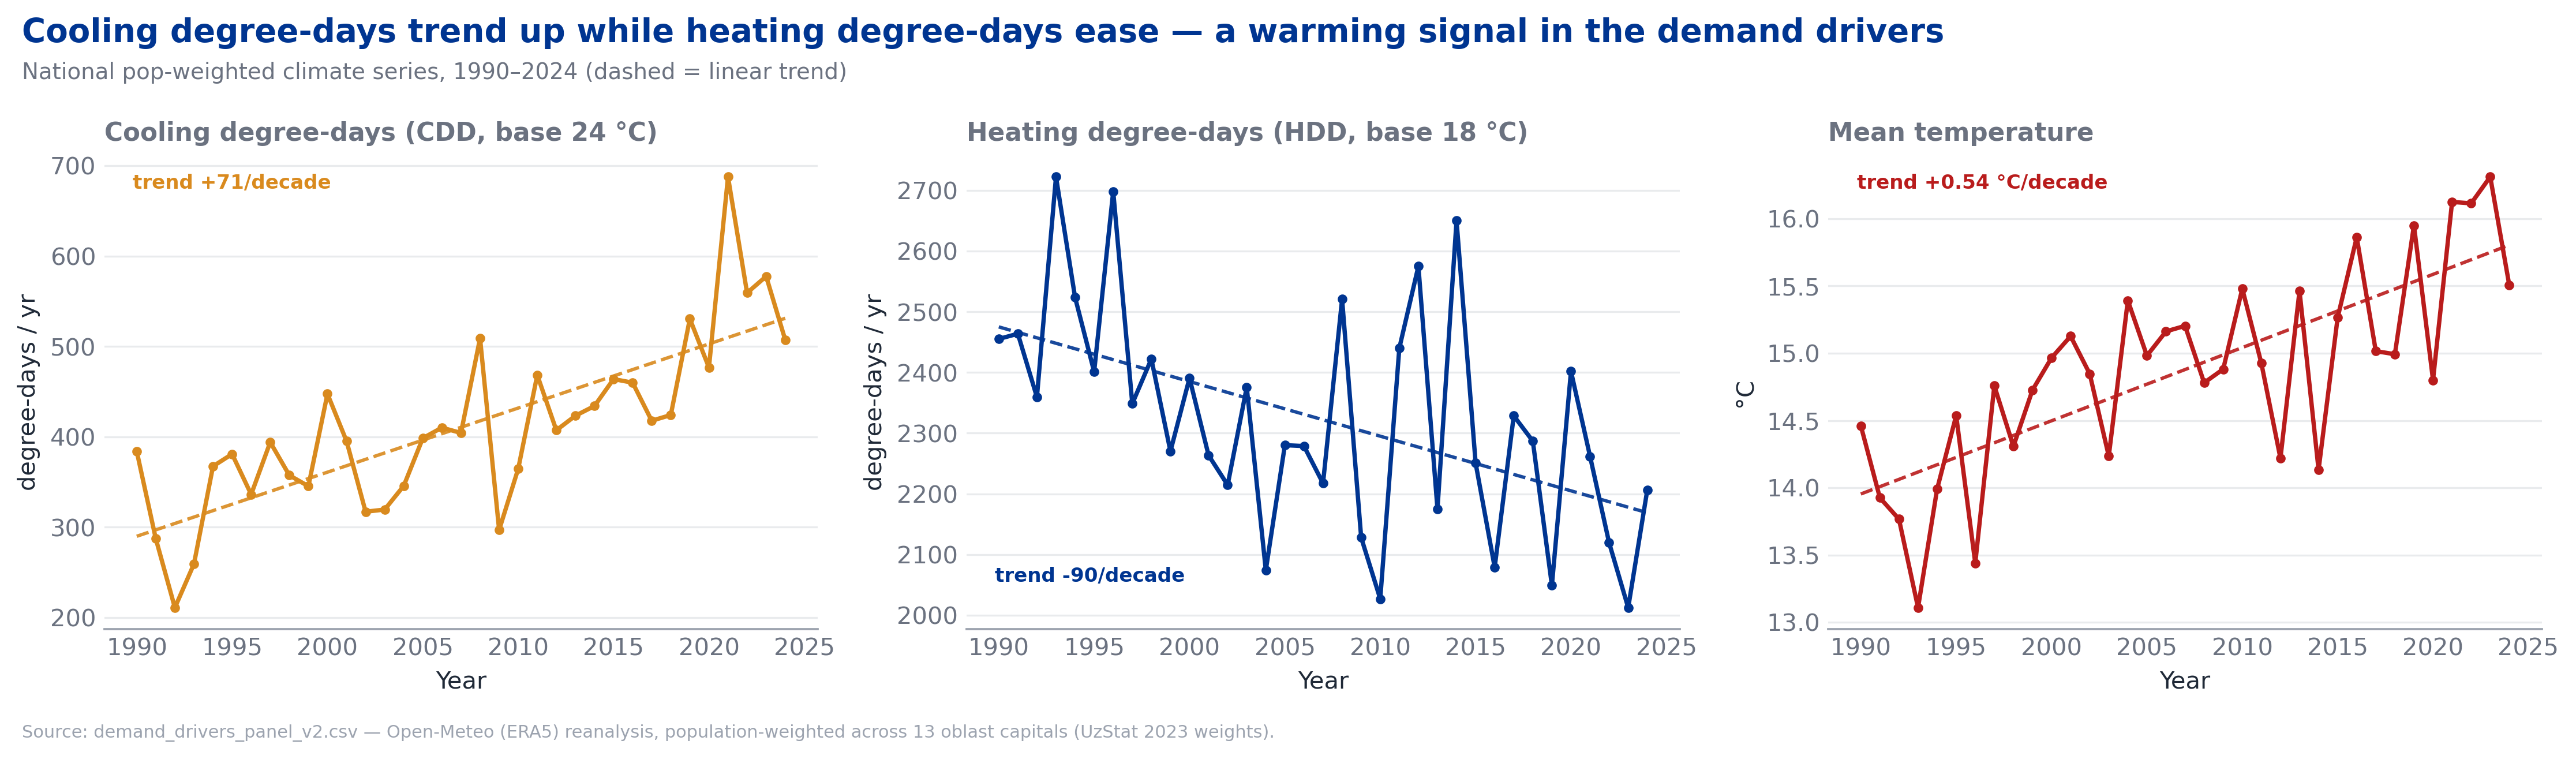
\includegraphics[width=\textwidth]{figures/climate_drivers.png}
\caption*{\itshape Figure 4.1. Population-weighted climate drivers, 1990--2024: cooling degree-days (base 24 $^\circ$C), heating degree-days (base 18 $^\circ$C) and mean temperature, each with its linear trend. Cooling degree-days trend up ($\sim$+71 per decade) as heating degree-days fall ($\sim$$-$90 per decade) on a mean-temperature rise of $\sim$0.54 $^\circ$C per decade --- the warming signal that makes cooling demand a growing structural driver. Source: demand\_drivers\_panel\_v2.csv, population-weighted across 13 oblast capitals (Open-Meteo, n.d.; StatSUZ, 2024).}
\end{figure*}

\subsection*{4.3 Baselines, the order of integration, and why there is no error-correction model}

\noindent The order of integration is settled by an augmented Dickey--Fuller
regression on the levels,
\begin{equation}
\Delta y_t=c+\gamma\,y_{t-1}+\textstyle\sum_{j}\delta_j\,\Delta y_{t-j}+\varepsilon_t,
\label{eq:adf}
\end{equation}
whose unit-root null $\gamma=0$ cannot be rejected (statistic $\approx+1.15$,
$p\approx0.996$), so the series is differenced once. The selected baseline is an
$\mathrm{ARIMA}(1,1,0)$, i.e. an AR(1) on the first difference,
\begin{equation}
(1-\phi_1 L)(1-L)\,y_t=c+\varepsilon_t
\;\Longleftrightarrow\;
\Delta y_t=c+\phi_1\,\Delta y_{t-1}+\varepsilon_t .
\label{eq:arima}
\end{equation}

The advanced models are required to beat an honest bench, so a ladder of baselines is fitted first, following standard forecasting practice (Hyndman \& Athanasopoulos, 2021): a naïve last-value carry-forward, a linear trend, a first-differenced regression, an AICc-selected ARIMA, Prophet, and a frequentist ridge\footnote{From the project's GitHub repository: forecast\_scoreboard\_baseline.csv (Notebook 06).}. The naïve model floors the bench at about 13.9\% error and the linear trend is worst at about 30.6\% --- predictably, because it ignores the series' integration order. The decision to difference once --- rather than twice, or not at all --- rests on three converging lines rather than the single test reported above: the unambiguous unit root in the levels; an AICc grid that, left free to choose, independently selects one order of differencing; and the parsimony argument that a second difference would over-smooth a thirty-point macro series and inflate forecast variance. The post-differencing diagnostics are genuinely mixed --- at twenty-eight points the differenced ADF still does not reject and KPSS now flips the other way --- and that ambiguity is reported rather than hidden, because it is the textbook small-sample artefact of a low-power test on a series dominated by one large 2017--18 jump (Box et al., 2015).

The same short sample is the reason this report stops short of an error-correction model, the standard tool for linking demand to its economic drivers in the long run. An error-correction model requires a cointegrating relationship estimated from the levels, and the test for one is badly underpowered at thirty observations; fitting it anyway would manufacture a long-run equilibrium the data cannot actually evidence. First-differencing and a lagged-demand term capture what the sample can genuinely support, and the report declines the false precision of the richer specification.

\subsection*{4.4 The honest scoring rule: ex-ante, not backcast}

\noindent \emph{Ex-ante} scoring forecasts each driver before the target and
feeds the demand lag from the model's own output, exactly as a live forecast
must:
\begin{equation}
\hat D_t=f\!\bigl(\hat{\mathbf{z}}_t,\ \hat D_{t-1}\bigr),\qquad t=T{+}1,\dots,T{+}h,
\label{eq:exante}
\end{equation}
where macro drivers follow a log random walk with drift,
$\ln\hat z_{t}=\ln z_{T}+(t-T)\,\hat g$, and climate is held at its recent
climatology. The conditional backcast instead substitutes the \emph{observed}
$\mathbf{z}_t$ and the \emph{true} $D_{t-1}$ --- the optimism the headline
declines. Models are scored by
\begin{equation}
\begin{aligned}
\mathrm{MAPE}&=\frac{100}{n}\sum_{i=1}^{n}\left|\frac{y_i-\hat y_i}{y_i}\right|,\\
R^{2}&=1-\frac{\sum_i (y_i-\hat y_i)^2}{\sum_i (y_i-\bar y)^2}.
\end{aligned}
\label{eq:scores}
\end{equation}
$R^{2}<0$ whenever the squared error exceeds the variance of the hold-out about
its own mean --- the model does worse than a flat line --- which is precisely
what the post-2018 break forces and what the table reports.

A driver-based model can be scored on the 2019--2023 hold-out in two very different ways, and the difference is the most important methodological choice in the report. The flattering way --- a conditional backcast --- feeds the model the \textit{observed} values of its drivers over the hold-out, so it is never asked to forecast its own inputs; this yields an impressive error of roughly 4--4.6\%. The honest way --- \textit{ex-ante} scoring --- forecasts each driver in turn (macro drivers as a log random walk with drift, climate from its recent climatology) and feeds the lagged-demand term recursively from the model's own predictions, exactly as a real forecast must. On that basis the single-country models' error rises to about 9--10\%. The gap between the two numbers is precisely the advantage a backcast quietly grants itself, and this report headlines the ex-ante figure and keeps the conditional one only as a labelled optimistic bound (Table 4.1, Figure 4.2). The earlier interim figures in the low single digits were conditional backcasts; they are not the headline.

The hold-out is, by design, a hard one. The 2019--2023 window contains the post-2018 demand surge --- roughly a 27\% jump over the 2018 level --- so any model trained only on 1990--2018 under-predicts it, and most post a \textbf{negative} hold-out R\textsuperscript{2}. The same five-year window also straddles the COVID-19 shock: Uzbek electricity consumption fell about 1.8\% in 2020 --- a contraction with no parallel in the surrounding 2015--2023 demand run-up --- before rebounding roughly 23\% in 2021. The hold-out therefore superimposes a transient pandemic dip on the post-2018 structural surge, two disturbances of opposite sign, neither of which a parsimonious model trained on the smooth pre-2019 record can anticipate; the pandemic distortion deepens the out-of-sample difficulty rather than relieving it, and is one more reason the headline $\sim$9--10\% ex-ante error is a hard-won figure rather than a pessimistic one. That negative score is the finding, not a flaw in the model: it measures how far the recent, policy-driven regime departs from any smooth extrapolation of the prior three decades, and demonstrates that no parsimonious model anticipates a structural break it was never shown. To keep the test clean, the ridge penalty is selected by expanding-window one-step-ahead cross-validation on the training years alone, never on the hold-out --- tuning a model on the data used to judge it would invalidate the comparison --- and standardisation is likewise fit on the training window only.

\begin{figure*}[tp]
\centering

\includegraphics[width=\textwidth]{figures/forecast_scoreboard_exante.png}
\caption*{\itshape Figure 4.2. The demand-model scoreboard on the single 2019--2023 hold-out. Bars show the ex-ante error each model incurs when it must forecast its own drivers and propagate the demand lag recursively; hollow markers show the conditional backcast on observed drivers, kept only as the optimistic reference. Single-country models cluster near 9--10\% with negative hold-out R\textsuperscript{2} against the deliberate post-2018 structural break; the pooled Central-Asia models lead at about 6\% and turn R\textsuperscript{2} positive. Source: forecast\_scoreboard\_advanced.csv (project Notebook 07).}
\end{figure*}

\begin{table*}[tp]
\centering
\caption*{\textbf{Table 4.1. Demand models on the 2019--2023 hold-out (single test window).} Ex-ante is the headline; the conditional backcast is reported for reference only. Model skill is scored by mean absolute percentage error (MAPE), read against conventional forecast-accuracy bands (Lewis, 1982).}
\renewcommand{\arraystretch}{1.18}\small
\begin{tabularx}{\textwidth}{LLrrr}
\toprule
\textbf{Model} & \textbf{Family} & \textbf{Ex-ante MAPE} & \textbf{Ex-ante R\textsuperscript{2}} & \textbf{Conditional MAPE \textit{(ref.)}} \\
\midrule
ARIMA(1,1,0) & time-series baseline & 9.2\% & $-$0.27 & --- \\
Ridge --- Uzbekistan (minimal) & single-country driver & 9.7\% & $-$0.66 & 4.6\% \\
Ridge --- Uzbekistan (extended) & single-country driver & 9.0\% & $-$0.37 & 4.0\% \\
Bayesian Ridge --- Uzbekistan (minimal) & single-country driver & 9.0\% & $-$0.39 & 4.4\% \\
\textbf{Bayesian Ridge --- Uzbekistan (extended) --- deployed} & single-country driver & 10.1\% & $-$0.84 & 4.3\% \\
Pooled Ridge --- 4 Central-Asia + fixed effects & pooled \textit{(validation)} & 6.1\% & +0.10 & 4.6\% \\
Pooled Bayesian Ridge --- 4 Central-Asia + fixed effects & pooled \textit{(validation)} & 6.2\% & +0.06 & 4.6\% \\
\bottomrule
\end{tabularx}
\par\smallskip{\footnotesize\itshape The ARIMA(1,1,0) --- a purely extrapolative model that uses no drivers, hence no conditional-backcast column --- posts the best ex-ante error in the table and edges the deployed driver model (9.2\% versus 10.1\%); on a five-point hold-out the two are statistically indistinguishable. It is nonetheless not the deployed model, for the reason \S{}4.5 sets out: a univariate time-series model cannot generate the driver-conditioned demand fan of Chapter 5 or the supply scenarios of Chapters 5--6 on which the advisory product rests. Exact figures: ARIMA 9.221\% / R\textsuperscript{2} $-$0.266; deployed Bayesian ridge 10.138\% / R\textsuperscript{2} $-$0.838 (project Notebook 06/07).}
\end{table*}

Figure 4.3 makes that negative R\textsuperscript{2} legible rather than abstract. It plots actual 2019--2023 demand against the ex-ante hold-out predictions of the four single-country driver models, each forecasting its own drivers and propagating the demand lag recursively. The actual series steps up sharply --- the post-2018 surge compounded by the 2021 rebound --- while every model, trained only on the smooth 1990--2018 record, tracks a far gentler path and under-shoots the 2023 actual by roughly \textbf{9 TWh, about 12\%}. The shortfall is not scatter around the actual but a one-sided gap below it, in the same direction for every model: that systematic under-prediction of a regime the training window never contained is exactly what a negative hold-out R\textsuperscript{2} against a structural break looks like.

\begin{figure*}[tp]
\centering
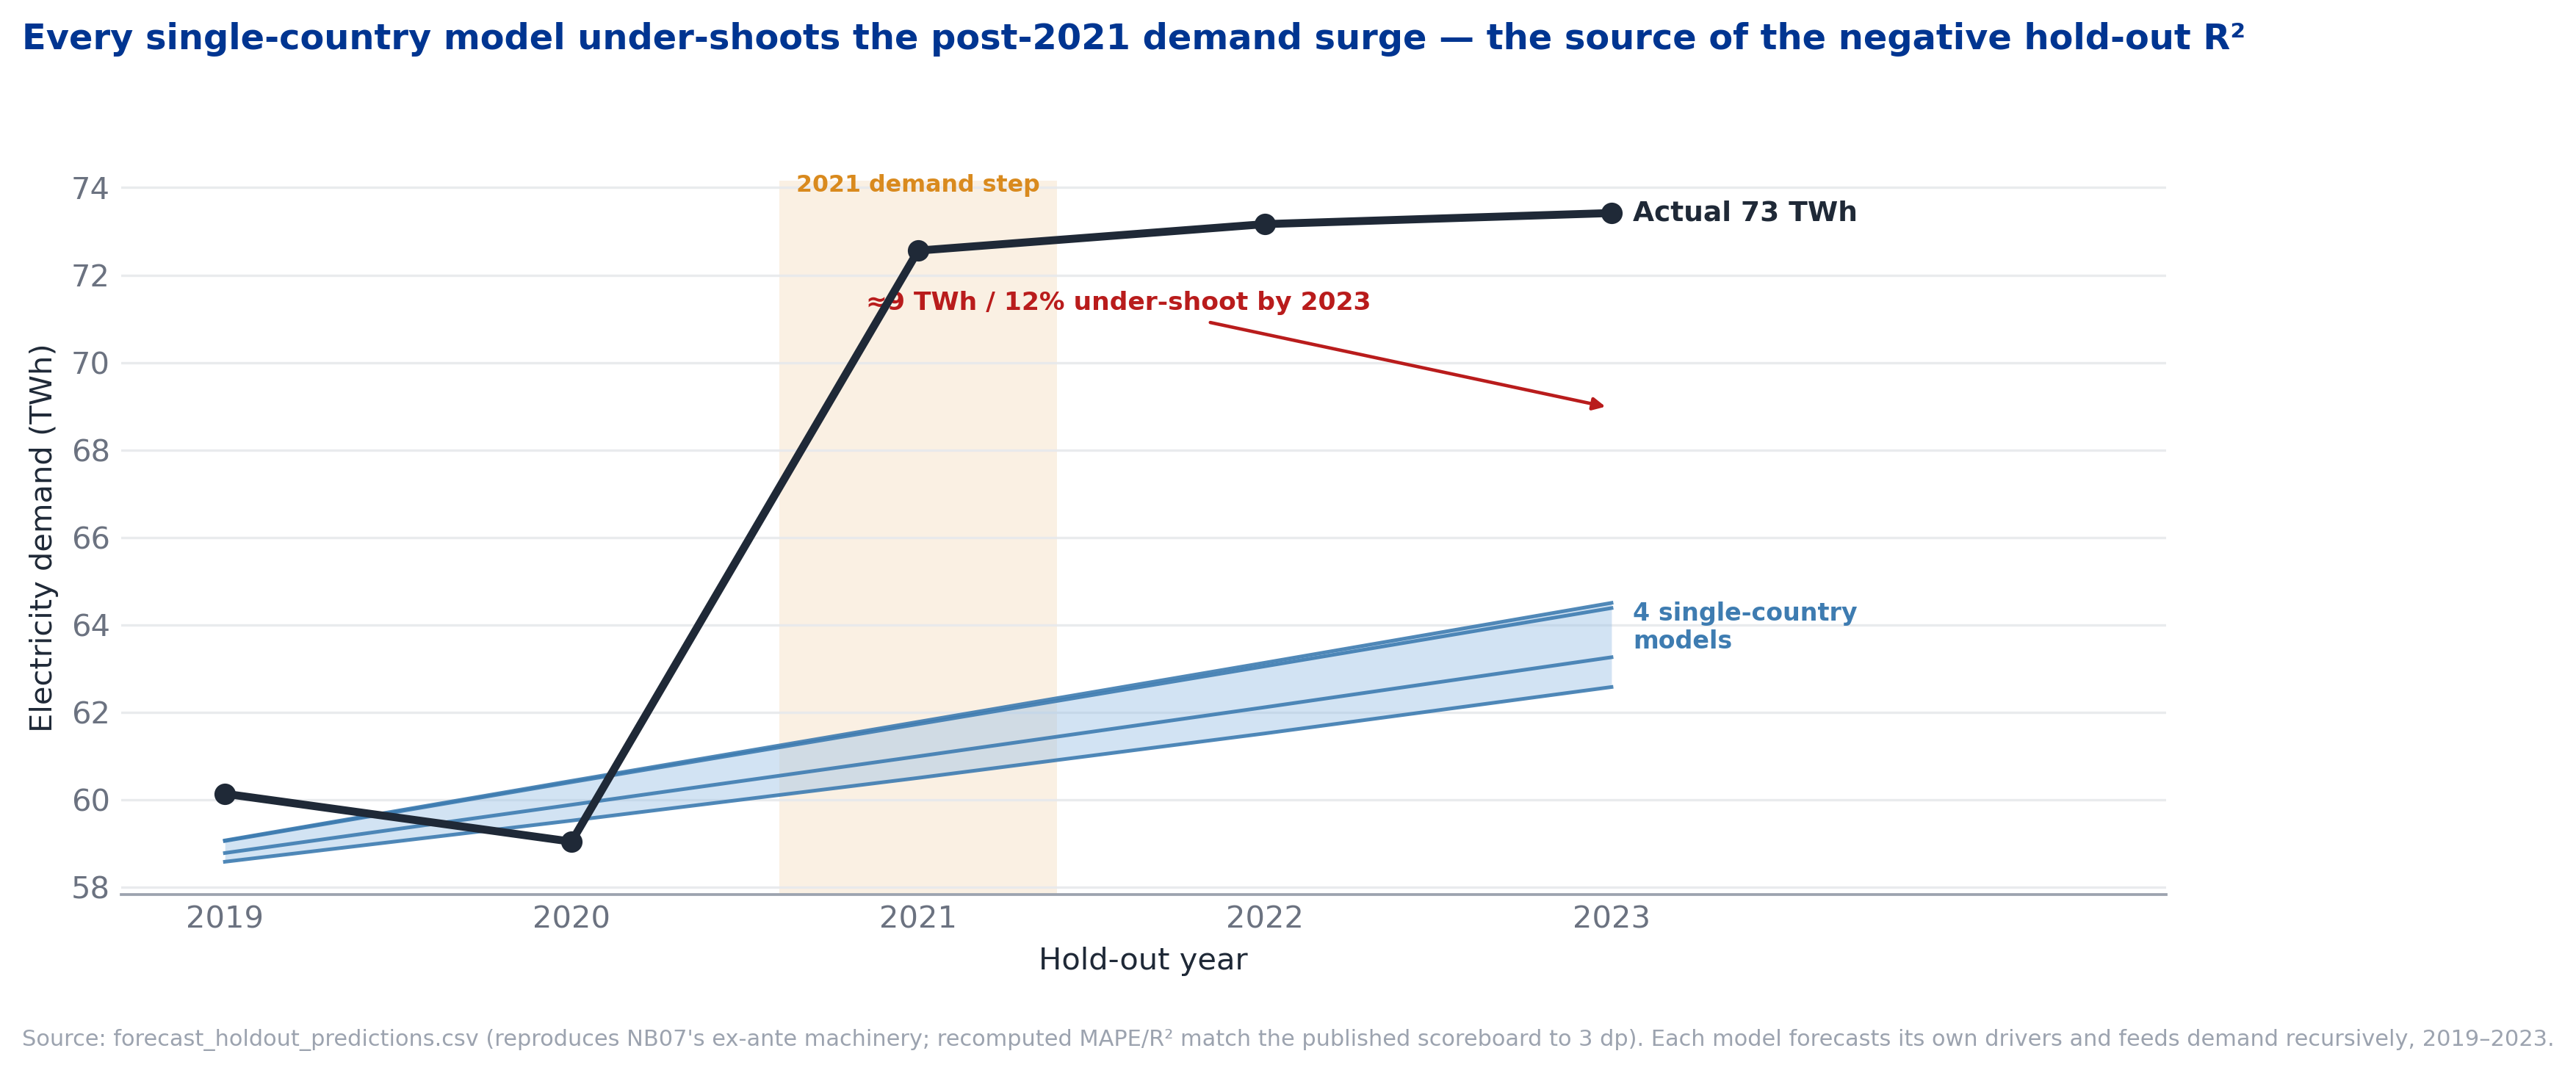
\includegraphics[width=\textwidth]{figures/forecast_holdout_actuals.png}
\caption*{\itshape Figure 4.3. Ex-ante hold-out --- actual electricity demand versus the four single-country models' 2019--2023 predictions. Each model forecasts its own drivers and propagates the demand lag recursively, so none is handed observed hold-out inputs; the shaded band spans the four models. All sit well below the post-2021 actual, under-shooting by $\sim$9 TWh ($\sim$12\%) at 2023 --- the visible source of the negative hold-out R\textsuperscript{2} in Table 4.1. Source: forecast\_holdout\_predictions.csv (reproduces the project Notebook 07 ex-ante machinery).}
\end{figure*}

\subsection*{4.5 Borrowing strength, and why the deployed model is the single-country one}

A negative hold-out R\textsuperscript{2} is the problem the rest of the method has to answer: thirty Uzbek points simply cannot span a regime they never contained. The answer is to widen the sample sideways. A pooled model is fitted across the four Central-Asian countries with complete driver coverage --- Kazakhstan, Kyrgyzstan, Tajikistan and Uzbekistan --- giving roughly ninety-five country-years against Uzbekistan's thirty-four, with Kazakhstan as the fixed-effect reference (Hsiao, 2014; IEA, 2024a). Turkmenistan, a structurally similar gas economy and in principle a useful peer, drops out because its macroeconomic series are incomplete --- a credible neighbour lost to data rather than excluded by choice, and named as such. Pooling rests on an explicit assumption: that the \textit{response structure} linking income, industry and climate to demand is broadly common across the region, while persistent \textit{level} differences between countries are absorbed by the country fixed effects. The payoff is decisive in the one place it matters --- the pooled models reach about 6\% ex-ante error with \textbf{positive} hold-out R\textsuperscript{2} (+0.06 to +0.10), because the borrowed country-years let the model observe income-driven demand growth that Uzbekistan's own history could not show it. The roughly ninety-five country-years available become about seventy-two once the hold-out is withheld, so the pool is wider than Uzbekistan's record but is itself still a small sample.

Pooling earns its keep, but a leave-one-country-out test shows precisely how far that keep extends --- and where it stops. Refitting the panel with one country wholly withheld and then predicting it from the other three turns the held-out error into a direct measure of how transferable the shared structure is. The results are uneven and instructive: the small hydro systems are predicted well from their neighbours (Tajikistan 8.1\%, Kyrgyzstan 11.7\% MAPE), while the large fossil systems transfer worst (Kazakhstan 23.4\%, Uzbekistan 19.6\%)\footnote{From the project's GitHub repository: leave-one-country-out cross-validation (Notebook 07 \S{}9.3).}. The reading is two-sided, and the report keeps both sides. Pooling validates the \textit{structure} --- a common income--industry--climate response does generalise across the region, which is what turns the pooled hold-out R\textsuperscript{2} positive --- but Uzbekistan is among the hardest countries in the panel to predict \textit{from the others}, so the pooled 6\% is a panel average that flatters the Uzbek-specific case rather than a promise that Uzbekistan has become easy to forecast. The pooled model corroborates the single-country one; it does not supersede it.

That the regularised-linear class is the right one is itself tested, not assumed. A gradient-boosted regression-tree ensemble (XGBoost) --- the one machine-learning model tested against the regularised-linear class --- scores far worse on the same pooled panel, about 13\% MAPE, because a high-variance learner cannot exploit ninety-odd country-years and over-reacts to Tajikistan's small, volatile system; and a SHAP decomposition of that tree independently reproduces the exploratory screen, attributing almost all explained demand to GDP per capita and industrial value-added and almost none to urbanisation, population or the country dummies (Lundberg \& Lee, 2017). The chain from the correlation analysis through feature selection to the fitted model is therefore internally consistent rather than merely asserted.

Why, then, is the deployed model a \textit{driver} model at all, when the best ex-ante score in Table 4.1 belongs to the ARIMA(1,1,0) --- 9.2\% against the deployed model's 10.1\%? The concession is granted plainly: on the five-point hold-out the ARIMA edges every driver specification, and the gap between it and the regressions is statistically meaningless on so short a window. Accuracy on the demand line is simply not the binding requirement. The advisory product is not a single demand number; it is the driver-conditioned predictive fan of Chapter 5 and the supply scenarios of Chapters 5 and 6, and \textbf{only a driver model can generate either.} A univariate ARIMA extrapolates demand from its own past and offers no channel through which income, climate, or a renewable build-out path can enter; it cannot be widened into a fan conditioned on macroeconomic scenarios, and it cannot be turned into a generation mix and a carbon-intensity path. The ARIMA wins the narrow contest and loses the deployable one --- it is reported as the honest extrapolative benchmark, and then set aside.

Among the driver models, the \textit{single-country} specification is deployed rather than the lower-error pooled one, for a reason of target rather than skill. The single-country models forecast the project's own reported series --- the bridged IEA--StatSUZ consumption path of Chapter 3 --- whereas the pooled models forecast the harmonised cross-country series, comparable across the four countries but defined on a different basis. The pooled model's 6\% is therefore earned on a different target; the cross-family comparison is indicative rather than exact, and a pooled number could not be reported as the Uzbek consumption path without reintroducing the boundary mismatch Chapter 3 worked to remove. So the single-country model is deployed because it forecasts exactly the series the report and dashboard carry, and the pooled model \textbf{validates} it --- its positive R\textsuperscript{2} and 6\% error are the external evidence, which the single-country hold-out cannot itself supply, that the structural relationship survives once the sample is widened. Among the four single-country specifications, all post negative R\textsuperscript{2} and cluster within a point of one another, so the break-dominated window cannot rank them --- and the ordering is not even internally consistent: the extended driver set \textit{improves} the plain ridge (9.7\% to 9.0\% ex-ante MAPE) yet slightly \textit{worsens} the Bayesian ridge (9.0\% to 10.1\%), the kind of incoherent flip that betrays a five-point test too short to separate the specifications. The deployment choice is therefore made on driver \textit{content}, not on that unrankable score. The minimal set carries only income, industrial value-added, urbanisation and the lagged-demand term; the extended set adds the three channels the exploratory screen validated as structural --- services value-added and the cooling- and heating-degree-day terms, the cooling term carrying Uzbekistan's genuine summer-load signal (\S{}4.2; project Notebook 07 \S{}3). These are not optional refinements. The advisory product is a \textit{driver-conditioned} demand fan, so the deployed model must itself forward-project demand through the income, sectoral and cooling channels --- climate from its recent climatology (\S{}4.4) --- to generate that fan; a specification that omits the cooling channel cannot, however marginally it scores on a window that cannot tell the specifications apart. The extended Bayesian ridge is deployed, then, because it carries the full validated structural driver set and returns the predictive standard deviation the Chapter 5 fan is built from --- not because it won a contest the hold-out is too short to decide.

\subsection*{4.6 From demand to supply, and what the method can and cannot deliver}

The advisory question is finally about supply --- renewable share, residual fossil generation and carbon intensity --- so the method closes the chain from the demand forecast through the generation mix to emissions, regenerated from the live model rather than from a retired snapshot. The supply scenarios are pinned to the deployed Bayesian-ridge baseline demand path: total generation is set to demand grossed up for grid losses, and the three scenarios then differ \textbf{only} in renewable build-out ambition, leaving demand uncertainty to the separate predictive fan. The capacity figures behind each scenario are taken from published targets or reported actuals, none invented. Two assumptions in this step are stated plainly because they shape the result. The forward grid-loss rate used to gross demand up into required generation is held at about 9\% --- a loss-\textit{reduction target}, well below the realized $\sim$16\% band (17.8\% in 2023) Chapter 3 documented; the two are not in conflict, but the gap between today's losses and the assumed target is itself an advisory signal, and Chapter 6 opens by reconciling the two and quantifying that gap as the system's modernization prize. And because the IMF World Economic Outlook drivers end in 2031, the 2032--2040 tail holds the terminal growth rate flat --- a transparent, growth-optimistic choice that lifts 2040 demand toward roughly 124 TWh and, by raising the denominator, makes the renewable-share targets \textit{harder} to reach. The three supply paths are therefore read as demanding policy envelopes, not point forecasts.

This is also where the limits of the method must be stated, not deferred. The probabilistic fan around the demand path combines the model's predictive standard deviation --- which captures parameter and residual uncertainty --- with three calibrated macro scenarios. It does \textbf{not} capture the error in forecasting the drivers themselves, the uncertainty of having chosen one model class over another, or the structural-break risk the hold-out so clearly exposed. The reported intervals are therefore best understood as \textbf{lower bounds} on the true uncertainty, not its full width. With that honestly marked, the division of labour for the rest of the report is set: the method can predict a demand path and attach a defensible, if conservative, band to it; it can only \textit{bound} the supply trajectories, which turn on policy and investment choices no statistical model can foresee. Chapter 5 turns this machinery on the data and reports what it produces.

\phantomsection\addcontentsline{toc}{section}{5 --- Forecasts and scenarios to 2040}\section*{5 --- Forecasts and scenarios to 2040}

\subsection*{5.1 How to read this chapter}

This chapter reports four things: a demand path to 2040, the probabilistic fan around it, and three supply scenarios that turn that demand into a renewable share, a residual fossil-generation path, and a grid carbon-intensity path. Each is presented the same way --- first what the exploratory analysis led the report to expect, then what the model actually produced, then whether the two agree. That ordering is deliberate. A forecast that merely confirms the descriptive chapters adds little; a forecast that contradicts them is either a discovery or a bug, and saying in advance what was expected is what makes the difference legible. Every result carries its caveat inline, where the number is, rather than in a footnote the reader can skip.

One framing point governs everything that follows. The demand path is a \textit{forecast} --- predicted, with a band. The three supply scenarios are \textit{not} forecasts; they are conditional projections that share the single demand path and differ only in how fast renewables are built (\S{}4.6). They are named for their build-out ambition --- \textbf{BAU}, \textbf{Government}, and \textbf{Accelerated} --- so that ``Accelerated'' never doubles as a demand-side label. Reading the scenario spread as a probability distribution over outcomes would misread it: it is a set of ``if-then'' envelopes, and the policy choice, not the data, decides which one the country lands on. Projecting a power system two decades forward from current policy and technology trajectories is the work of the long-horizon energy-transition outlook (DNV, 2025); this report applies that horizon to a single, data-constrained country rather than to the global system.

\subsection*{5.2 The demand path}

\keystat{Demand to 2040}{74 $\rightarrow$ 86 $\rightarrow$ 124 TWh}%
{Electricity demand rises about 2.5\% a year to 2030, then climbs further on a
deliberately growth-optimistic terminal tail held flat from 2031 ($\S$5.2).}

The exploratory analysis predicted that electricity demand would keep climbing and that income would be the engine: demand, GDP per capita, industrial and services value-added all trend upward almost in lockstep (mutually correlated at \textit{r} $\approx$ 0.99, \S{}4.2), and cooling demand adds a genuine summer-load signal on top. Nothing in the data suggested demand was near saturation. The forecast bears this out without surprise (Figure 5.1). The deployed extended Bayesian-ridge model projects demand rising from \textbf{73.98 TWh in 2024 to 86.01 TWh in 2030} --- about 2.5\% a year, accelerating across the window as the income drivers compound --- and then, on the held-flat terminal-growth tail that begins where the IMF driver path ends in 2031 (\S{}4.6), continuing to roughly \textbf{123.9 TWh by 2040} (project Notebook 07 \S{}8; IMF, 2026). These figures match the dataset's own most recent anchor: the bridged 2024 demand of about 77.7 TWh on the IEA-consumption basis of \S{}3.4 and the model's 73.98 TWh starting value are the same quantity read on two boundaries, and the report does not blur them.

The 2040 figure should be read as the deliberately growth-optimistic end of a plausible range, not a central expectation. Holding the terminal growth rate flat across 2032--2040 is a transparent assumption that lifts demand rather than letting it taper, and it has a specific consequence the next sections rely on: a higher demand denominator makes every renewable-\textit{share} target harder to reach, so the scenarios are tested against a demanding load, not a flattering one.

\begin{figure*}[tp]
\centering

\includegraphics[width=\textwidth]{figures/forecast_demand_bayes_ridge.png}
\caption*{\itshape Figure 5.1. Deployed demand forecast, 2024--2030, from the extended Bayesian-ridge model, with the 90\% predictive band. Demand rises from 73.98 TWh (2024) to 86.01 TWh (2030); the 90\% band widens from [66.4, 81.6] to [76.7, 95.3] TWh. The band is the model's own predictive standard deviation and is a lower bound on true uncertainty (\S{}5.3). The shaded 2020--21 band marks the COVID-19 demand shock --- a $\sim$1.8\% dip in 2020 followed by a sharp 2021 rebound, retained rather than smoothed because it is part of why the 2019--2023 hold-out is hard (\S{}4.4). Source: forecast\_demand\_bayes\_ridge.csv (project Notebook 07 \S{}8).}
\end{figure*}

\subsection*{5.3 The fan, and why it is a lower bound}

The exploratory work gave no reason to expect a tight forecast --- thirty observations, a structural break in 2017--18, and drivers that must themselves be projected all argue for a wide band --- and the fan is correspondingly wide. At 2030 the model's 90\% predictive band runs from \textbf{76.7 to 95.3 TWh} around the 86.0 central value (roughly $\pm$11\%); extended to 2040 the published fan reaches \textbf{[110, 137] TWh at 80\% and [103, 145] TWh at 95\%} confidence\footnote{From the project's GitHub repository: forecast\_demand.csv (Notebook 07 \S{}8).}.

What matters more than the width is what the width does \textit{not} include, and this is stated wherever the fan appears. The band is built from the model's predictive standard deviation --- parameter and residual uncertainty --- combined with the macro scenarios. It does not propagate the error in forecasting the drivers themselves, the recursive-lag error that compounds as each year's prediction feeds the next, or the model-choice and structural-break risk the negative hold-out R\textsuperscript{2} exposed (\S{}4.4). The reported intervals are therefore \textbf{lower bounds} on the true uncertainty. A reader who treats the 95\% band as a genuine 95\% interval will be overconfident; the honest claim is narrower --- that the true uncertainty is \textit{at least} this wide.

\subsection*{5.4 From demand to generation: one path, three mixes}

\noindent Demand is grossed up to required generation at the forward
loss-reduction target $\ell\approx0.09$ ($\S6.1$),
\begin{equation}
G_t=D_t\,(1+\ell),
\label{eq:gross}
\end{equation}
giving the single generation path shared by all three scenarios
($80.6\rightarrow135.1$ TWh). Each renewable technology's output is its capacity
times an annualised capacity factor, and thermal is the residual that closes the
balance:
\begin{equation}
G_{k,t}=\mathrm{CF}_k\cdot \mathrm{Cap}_{k,t}\cdot 8760,\quad
G_{\mathrm{th},t}=G_t-\!\!\sum_{k\neq\mathrm{th}}\!\! G_{k,t},
\label{eq:mix}
\end{equation}
for $k\in\{\text{solar},\text{wind},\text{hydro}\}$, with the renewable share
$s_t=\bigl(\sum_{k\in\mathrm{RE}}G_{k,t}\bigr)/G_t$.

The supply scenarios begin by converting demand into the generation that must be dispatched to meet it. That conversion grosses demand up for grid losses at the forward target rate of about 9\% (the loss-reconciliation Chapter 6 opens with), so total generation runs from \textbf{80.6 TWh in 2024 to 93.8 TWh in 2030 and 135.1 TWh in 2040} --- and this single generation path is \textbf{identical across all three scenarios}\footnote{From the project's GitHub repository: scenario engine, forecast\_scenarios.csv (Notebook 07 \S{}8).}. The scenarios diverge only in how that fixed total is split among thermal, hydro, solar, and wind. Holding the total constant is what isolates the one variable of interest --- build-out ambition --- from demand uncertainty, which lives entirely in the separate fan of \S{}5.3. It also means the scenario spread says nothing about whether demand is high or low; it speaks only to the mix.

\subsection*{5.5 Renewable share}

\keystat{BAU renewable share}{43\% (2030) $\rightarrow$ 36\% (2040)}%
{A build-out that is not sustained does not merely stall the transition --- it
\emph{reverses} it, ceding the post-2030 demand increment back to gas ($\S$5.5).}

Chapter 2 predicted that the renewable share could rise only as fast as new solar and wind are built, because hydropower is already fully used and gas cannot decarbonise itself --- decarbonisation here is a construction story, not a re-dispatch. The scenarios make that prediction quantitative, and they bear it out with one important nuance (Figure 5.2). From a 2024 base, the renewable share by 2030 reaches \textbf{43.1\% under BAU, 58.4\% under Government, and 70.8\% under Accelerated}; by 2040 the three diverge sharply --- \textbf{36.5\%, 60.0\%, and 80.0\%} respectively\footnote{From the project's GitHub repository: scenario engine, forecast\_scenarios.csv (Notebook 07 \S{}8).}. The nuance is the BAU trajectory: its share \textit{peaks} near 2030 and then \textit{declines}, because in BAU the contracted solar-and-wind pipeline is completed but not extended, so once demand keeps climbing after 2030 the system meets the increment by burning more gas, and the renewable share slides backward. A build-out that is not sustained does not merely stall the transition; it reverses it.

A caution on the base year belongs here, inline --- and it resolves cleanly once the construction is understood. The scenario engine does not start from a 2024 share and add increments; it builds each year's renewable share from that year's \textit{capacity targets multiplied by a technology capacity factor}. The 2024 value this produces --- about 22.6\% total renewables (10.3\% non-hydro) --- runs \textit{higher} than the independently sourced figure Chapter 2 reports for the same year (about 16\% total, under 6\% non-hydro, OWID/Ember basis), because the reconstruction credits newly commissioned 2024 plant with a full year of output it did not physically run. That makes the 2024 base a partial-year artifact. Crucially, because every later share is computed forward from the 2030 capacity targets rather than carried up from 2024, the artifact \textbf{does not propagate}: the 2030 and 2040 shares --- and the \S{}5.8 verdicts that rest on them --- are unaffected (BAU, for instance, clears the 40\% generation target down to a solar capacity factor of about 0.145, so its margin is structural, not an artefact of the base). The absolute 2024 base is the one number not to quote on its own; the trajectories and the inter-scenario spread are sound.

\begin{figure*}[tp]
\centering

\includegraphics[width=\textwidth]{figures/forecast_scenarios.png}
\caption*{\itshape Figure 5.2. Generation mix and renewable share under the three supply scenarios, 2024--2040. All three share one total-generation path (80.6 $\rightarrow$ 135.1 TWh) and differ only in build-out. The renewable share reaches 43.1\% / 58.4\% / 70.8\% by 2030 (BAU / Government / Accelerated) and 36.5\% / 60.0\% / 80.0\% by 2040; note the BAU share peaks near 2030 and then declines as unsustained build-out cedes the demand increment back to gas. Source: forecast\_scenarios.csv (project Notebook 07 \S{}8).}
\end{figure*}

\subsection*{5.6 Residual fossil generation}

The same logic, read on the fossil side, produces the sharpest single number in the chapter. Chapter 2 observed that demand growth had historically been met by burning more gas, with thermal output growing about 2.5\% a year while hydro flatlined. The scenarios show that pattern either breaking or continuing, depending entirely on build-out. Thermal generation, \textbf{62.4 TWh in 2024}, falls under every scenario to 2030 (to 53.3, 39.0, and 27.4 TWh under BAU, Government, and Accelerated) --- but then the paths split violently. By 2040 thermal generation is \textbf{85.8 TWh under BAU --- higher than today} --- against 54.0 TWh under Government and a flat \textbf{27.0 TWh under Accelerated}\footnote{From the project's GitHub repository: scenario engine, forecast\_scenarios.csv (Notebook 07 \S{}8).}. The BAU result is the one to dwell on: it is not that decarbonisation merely stalls, but that absolute fossil generation in 2040 \textit{exceeds} the 2024 level, because a rising demand denominator with a frozen renewable build forces more gas through the system than runs through it today. The transition is not self-sustaining; left to the completed pipeline alone, the fossil fleet grows.

\subsection*{5.7 Carbon intensity}

\noindent Grid carbon intensity is the generation-weighted emission factor, and
annual power-sector emissions follow by multiplication:
\begin{equation}
I_t=\frac{\sum_k G_{k,t}\,\mathrm{EF}_k}{G_t}\;\bigl[\text{gCO}_2/\text{kWh}\bigr],
\qquad
\mathrm{CO}_{2,t}=I_t\,G_t,
\label{eq:carbon}
\end{equation}
with $\mathrm{EF}_{\mathrm{th}}$ the gas-weighted thermal factor
(88\% gas / 12\% coal) and $\mathrm{EF}_k=0$ for solar, wind and hydro.

Grid carbon intensity follows mechanically from the mix. The exploratory analysis measured the historical grid at about \textbf{668 gCO\textsubscript{2}/kWh in 2023} --- within a 590--825 gCO\textsubscript{2}/kWh range across the record, settling to roughly 590--680 from 2018 onward as the fuel mix held steady (project Notebook 03 \S{}8). The scenario engine, however, reconstructs a 2024 starting intensity of about \textbf{520--530 gCO\textsubscript{2}/kWh} --- some 140 g below the EDA's own 2023 measurement, a one-year drop of roughly a fifth that the physical system did not undergo. The seam has the same origin as the renewable-share base discussed in \S{}5.5: the scenario's 2024 mix is implied from capacity figures rather than read from the metered generation series, so it understates the gas share in the partial-year base. The scenario \textit{paths} are nonetheless sound, because each later year's intensity is built forward from that year's generation mix --- and from 2030 onward the mix is set by published capacity targets, not by the 2024 base --- so the artifact is a base-year seam that does not propagate into the 2030 and 2040 figures. Read forward from that reconstructed base, the scenarios drive intensity in three directions (Figure 5.3). By 2030 carbon intensity falls to \textbf{390 gCO\textsubscript{2}/kWh under BAU, 245 under Government, and 172 under Accelerated}; by 2040 the spread is enormous --- \textbf{436, 179, and 90 gCO\textsubscript{2}/kWh} respectively\footnote{From the project's GitHub repository: scenario engine, forecast\_co2.csv (Notebook 07 \S{}8).}. The BAU path again bends the wrong way after 2030: intensity \textit{rises} from 390 back to 436 gCO\textsubscript{2}/kWh as thermal generation regrows, so the business-as-usual grid in 2040 is dirtier per kilowatt-hour than it was in 2030. In absolute terms, annual power-sector CO\textsubscript{2} runs from about 42--43 Mt in 2024 to \textbf{58.9 Mt (BAU), 24.2 Mt (Government), and 12.1 Mt (Accelerated) in 2040}\footnote{From the project's GitHub repository: scenario engine, forecast\_co2.csv (Notebook 07 \S{}8).}. The gap between the BAU and Accelerated endpoints --- a factor of nearly five in carbon intensity --- is the whole stake of the transition expressed in one comparison, and it is decided by build-out policy, not by anything the demand forecast can settle.

\begin{figure*}[tp]
\centering

\includegraphics[width=\textwidth]{figures/forecast_co2.png}
\caption*{\itshape Figure 5.3. Power-sector carbon intensity (gCO\textsubscript{2}/kWh) under the three scenarios, 2024--2040. From a reconstructed 2024 base of $\sim$520--530 gCO\textsubscript{2}/kWh --- below the $\sim$668 gCO\textsubscript{2}/kWh the exploratory analysis metered for 2023 (\S{}5.7) --- intensity reaches 390 / 245 / 172 by 2030 and 436 / 179 / 90 by 2040 (BAU / Government / Accelerated). BAU intensity rises after 2030 as thermal regrows. The dotted reference marks the $\sim$445 gCO\textsubscript{2}/kWh world-average power-sector carbon intensity (IEA, 2024e). Source: forecast\_co2.csv (project Notebook 07 \S{}8).}
\end{figure*}

\subsection*{5.8 The scenarios against the legislated targets}

\keystat{2040 power-sector carbon intensity}{436 vs 90 gCO\textsubscript{2}/kWh}%
{The BAU-versus-Accelerated spread is nearly fivefold, and it is decided by
build-out policy, not by anything the demand forecast can settle ($\S$5.7).}

Set beside Uzbekistan's own targets, the scenarios reveal which commitments are easy and which are binding. The legislated goal is a 40\% renewable \textit{generation} share and roughly 27 GW of renewable \textit{capacity} by 2030, with the presidency aspiring to a 54\% share (\S{}1.2). On the generation-share test, the results are almost anticlimactic: \textbf{all three scenarios clear 40\% by 2030} --- even BAU, at 43.1\% --- so the headline share target is not, on these projections, the demanding constraint. The harder tests are two. First, the \textit{capacity} target: total renewable capacity at 2030 reaches about \textbf{18 GW under BAU, 24.7 GW under Government, and 30.2 GW under Accelerated}, so only the Accelerated build meets the 27 GW commitment, and the Government path falls modestly short\footnote{From the project's GitHub repository: capacity columns of forecast\_scenarios.csv (Notebook 07 \S{}8).}. Second, and more revealing, \textit{sustaining} the share past 2030: only the Government and Accelerated paths hold or extend it, while BAU surrenders it. The presidential 54\% aspiration, for its part, is reached by 2030 only under the Government and Accelerated builds, not BAU. The advisory reading is clean: the 2030 share headline will likely be met on momentum, but the capacity target and the post-2030 trajectory are where ambition actually has to be financed --- and that is precisely where Chapter 6 locates the opportunity.

\phantomsection\addcontentsline{toc}{section}{6 --- Investment signals and advisory opportunity}\section*{6 --- Investment signals and advisory opportunity}

\subsection*{6.1 The loss-rate reconciliation, and the prize it defines}

\keystat{T\&D losses: realized vs target}{$\sim$16\% vs $\sim$9\%}%
{About seven percentage points of throughput is lost above what a modernised
network would lose --- the single largest efficiency prize in the data ($\S$6.1).}

One number must be reconciled before any signal in this chapter can be read, because two very different versions of it circulate through the project. Uzbekistan's realized transmission-and-distribution losses are chronic and high: the post-2001 record sits in a 13--18\% band every year, the five-year rolling mean stands at \textbf{16.3\%}, and the most recent confirmed figure is \textbf{17.8\% in 2023} (\S{}3.6) (World Bank, 2024; EDB, 2026). The competing \textbf{$\sim$9\%} figure that appears in the project's forward conversion and in some early captions is \textit{not} a measurement of today's grid --- it is two different things wearing the same digits: the pre-2001 narrow-basis loss series (\S{}3.6), and the government's forward loss-\textit{reduction target} used to gross demand up into generation (\S{}4.6 and \S{}5.4). Holding these apart is the whole point. The realized rate is $\sim$16\%; the target is $\sim$9\%; and \textbf{the gap between them is the modernization prize.} Roughly seven percentage points of the energy entering Uzbekistan's grid is lost above what a modernised network would lose --- energy that is generated, often by burning imported-grade gas, and then never billed. Closing that gap is simultaneously a decarbonisation lever, a cost recovery, and a deferral of new generation, and it is the single largest efficiency opportunity the data points to (Figure 6.1).

\begin{figure*}[tp]
\centering

\includegraphics[width=\textwidth]{figures/eda_td_losses.png}
\caption*{\itshape Figure 6.1. Transmission-and-distribution losses, 1990--2023. The series steps from $\sim$9\% before 2001 to a 13--18\% band thereafter --- a change in accounting basis, not a real doubling (\S{}3.6) --- and the modern record stays chronically near 16\%, reaching 17.8\% in 2023. The forward conversion target of $\sim$9\% (\S{}5.4) is a policy goal, not the realized rate; the gap is the modernization opportunity of \S{}6.5. Source: investment\_signal\_td.csv (project Notebook 08).}
\end{figure*}

\subsection*{6.2 Signal 1 --- Reserve headroom, not a forecast deficit}

The first signal must be stated carefully, because its construction invites an overclaim the report declines to make. The deficit analysis compares required generation (demand grossed up for losses) against planned supply --- but planned supply is \textit{set equal} to the central required generation, so at the central demand path the system balances by construction and the point deficit is zero in every year\footnote{From the project's GitHub repository: investment-signal model, investment\_signal\_deficit.csv (Notebook 08).}. There is therefore no forecast ``supply gap'' along the central path, and the report does not claim one. The genuine signal is the \textbf{reserve headroom the demand uncertainty implies}: at the upper-80\% demand band, required generation exceeds the central plan by about \textbf{6.5 TWh in 2024, widening to 14.8 TWh by 2040}\footnote{From the project's GitHub repository: investment-signal model, investment\_signal\_deficit.csv (Notebook 08).}. That is the capacity margin the build-out must carry to stay adequate against a plausibly higher load --- a reserve-planning quantity, identical across the three scenarios because it is driven by the shared demand fan rather than by build-out ambition. The year-by-year ``deficit/stress'' flags in the underlying table alternate on rounding noise around a zero point estimate and should not be read as a calendar of shortfalls; the substantive number is the widening reserve requirement.

\subsection*{6.3 Signal 2 --- Gas-import exposure}

The second signal makes Chapter 2's gas-dependence concrete and forward-looking. Gas burned for power generation stands at about \textbf{17 bcm in 2024}, and its 2040 value is a direct function of build-out: it \textbf{rises to 24.3 bcm under BAU}, falls to about \textbf{8.9 bcm under Government} and stays roughly flat thereafter, and falls further to about \textbf{4.5 bcm under Accelerated}, declining steadily through 2040 (gas is assumed to supply 88\% of thermal output)\footnote{From the project's GitHub repository: investment-signal model, investment\_signal\_gas.csv (Notebook 08).}. The exposure this measures is both fiscal and strategic: Uzbekistan is a net gas exporter that turns net importer in winter (\S{}2.6), so every bcm burned for domestic power is a bcm not exported and, at the winter margin, a bcm imported. The BAU path therefore does not merely emit more carbon; it deepens the country's exposure to gas-price and gas-supply shocks at exactly the season the grid is tightest, while the Accelerated path cuts gas-for-power by roughly three-quarters and insulates the system. Renewable build-out reads, in this signal, as energy-security policy as much as climate policy.

That power-sector draw lands on a national gas balance that is itself tightening, and the wider picture sharpens the signal (Figure 6.2). On the StatSUZ energy-balance basis, gas production has slid from comfortably above domestic demand --- a self-sufficiency ratio of about \textbf{125\% in 2010} --- to roughly \textbf{88\% in 2024}, with output dropping below domestic consumption for the first time around \textbf{2023}. The country that built its power system on cheap surplus gas now sits, on its own production trend, below self-sufficiency. This is the macro fact beneath the power-sector exposure above: once the overall balance crosses under 100\%, every incremental bcm the BAU grid burns for electricity is drawn from a pool that no longer covers domestic needs, so the fiscal cost and the winter-supply risk both bind harder than the power-sector figures alone suggest. Renewable build-out, read against this trend, is the most direct lever the power sector has on national gas security.

\begin{figure*}[tp]
\centering
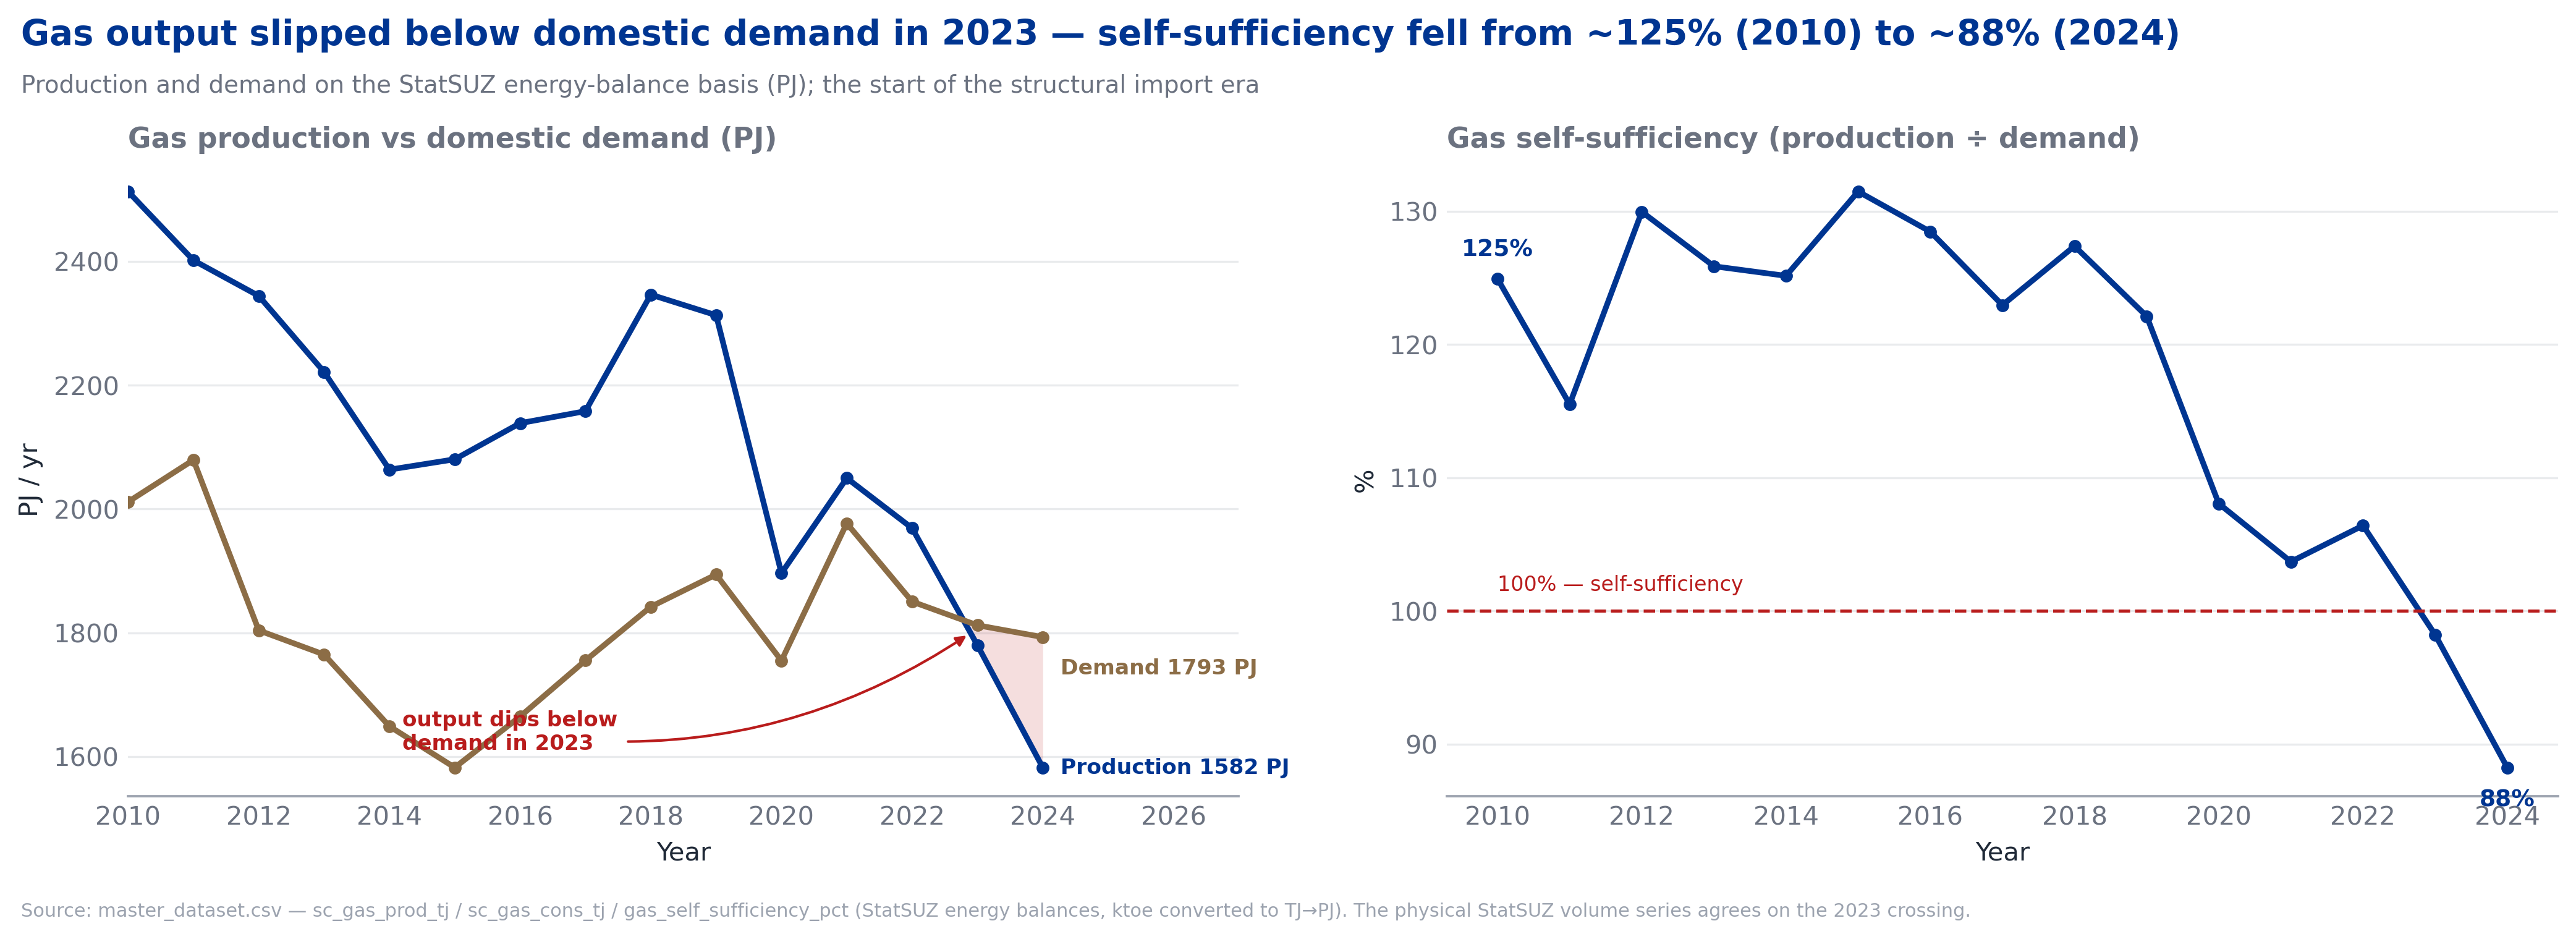
\includegraphics[width=\textwidth]{figures/gas_production_consumption.png}
\caption*{\itshape Figure 6.2. National gas production versus domestic demand (left, PJ) and the self-sufficiency ratio (right, production ÷ demand), on the StatSUZ energy-balance basis, 2010--2024. Self-sufficiency falls from $\sim$125\% in 2010 to $\sim$88\% in 2024, crossing below 100\% around 2023 --- the onset of structural import exposure at the margin. Source: master\_dataset.csv, StatSUZ energy balances (ktoe$\rightarrow$TJ$\rightarrow$PJ) (StatSUZ, 2024).}
\end{figure*}

\subsection*{6.4 Signal 3 --- The persistence of grid losses}

The third signal is the loss rate of \S{}6.1 read as a \textit{trend} rather than a level: losses have not merely been high, they have been stubbornly stable near 16\% for two decades, with no downward trajectory in the confirmed record (Figure 6.1)\footnote{From the project's GitHub repository: investment-signal model, investment\_signal\_td.csv (Notebook 08).}. Persistence is itself the signal. A loss rate that drifted down would suggest the problem is being solved by incremental maintenance; a loss rate pinned at 16\% across twenty years of rising demand indicates chronic underinvestment in transmission and distribution that ordinary operations will not fix. This is the demand-side complement to the supply-side opportunity: the same network that loses a sixth of its throughput is the network that must absorb a west-to-east renewable build and a five-fold swing in possible 2040 carbon intensity. The persistence finding is what turns grid modernization from a maintenance line item into a structural advisory engagement.

\subsection*{6.5 Capital envelopes, mapped to the advisory categories}

The signals above imply capital, and the model sizes it --- with a caveat that must travel with every figure. The capex numbers are \textbf{undiscounted, constant-cost upper-bound envelopes}: unit costs multiplied by capacity added, with no discounting, no learning-curve cost decline, and no financing structure. They bound the capital mobilised; they are not net-present-value estimates, and they should be read as the high end of a range\footnote{From the project's GitHub repository: investment-signal model, investment\_signals.csv (Notebook 08).}. On that basis the total 2024--2040 build-out envelope is about \textbf{\$27.3 bn under BAU, \$56.9 bn under Government, and \$79.3 bn under Accelerated}, with wind and solar the largest line items in every scenario (Government: wind \$16.0 bn, solar \$13.1 bn, thermal \$12.1 bn, hydro \$8.4 bn, transmission \$6.2 bn, storage \$1.1 bn)\footnote{From the project's GitHub repository: investment-signal model, investment\_signals.csv (Notebook 08).} (Figure 6.3).

\begin{figure}[tbp]
\centering

\includegraphics[width=\columnwidth]{figures/forecast_investment.png}
\caption*{\itshape Figure 6.3. Capital envelope by technology and scenario, 2024--2040 (undiscounted, constant-cost upper bounds). Total build-out runs $\sim$\$27.3 bn (BAU), $\sim$\$56.9 bn (Government), $\sim$\$79.3 bn (Accelerated); wind and solar dominate. Source: investment\_signals.csv (project Notebook 08).}
\end{figure}

Mapped to the five categories through which an engineering-advisory practice would engage, the Government-path programme falls out as follows (project Notebook 08 \S{}15):

\begin{table*}[tp]
\centering
\renewcommand{\arraystretch}{1.18}\small
\begin{tabularx}{\textwidth}{lLLr}
\toprule
\textbf{\#} & \textbf{Advisory category} & \textbf{What it covers} & \textbf{Indicative envelope} \\
\midrule
1 & \textbf{Generation build} & $\sim$25 GW of new renewable capacity to the government target & $\sim$\$28 bn \\
2 & \textbf{Grid modernization} & $\sim$6,000 km of HV lines plus a $\sim$1,450 km wind-corridor evacuation, and the loss-reduction programme of \S{}6.1 & $\sim$\$3.0 bn \\
3 & \textbf{Renewable integration} & balancing and storage ($\sim$5 GWh BESS) to absorb a $\ge$40\% variable share & $\sim$\$2.0 bn \\
4 & \textbf{Energy efficiency (NEEA)} & tariff reform and demand-side efficiency & $\sim$\$1.5 bn \\
5 & \textbf{PPP / IFI advisory} & structuring the EBRD / ADB / IFC project pipeline & advisory fees \\
\bottomrule
\end{tabularx}
\par\smallskip{\footnotesize\itshape The category figures are NB08's curated advisory cut and rest on a slightly different basis than the technology envelope above (for instance, the $\sim$\$28 bn generation line is close to, but not identical with, the scenario's combined solar-and-wind capex); both are upper-bound envelopes and the two cuts are not meant to reconcile to the dollar.}
\end{table*}

The mapping is the chapter's payoff. Generation build is the largest envelope but also the most contested commercially; grid modernization and renewable integration are smaller in dollars but are where the loss-persistence and reserve-headroom signals make engagement close to unavoidable; and the efficiency and PPP-structuring categories are where advisory fees, rather than capital, accrue. The opportunity is not uniform across the programme --- it concentrates exactly where the structural signals are sharpest.

\subsection*{6.6 Plan B --- firm low-carbon capacity at Jizzakh}

One contingency sits outside the three renewable scenarios and is modelled as a parametric overlay rather than folded into the baseline, because its construction has only just begun and Central Asia has no commissioning precedent. The Jizzakh nuclear plant --- a 2.1 GW integrated station pairing two VVER-1000 reactors with two RITM-200N small modular units (\S{}2.4) --- would add firm, dispatchable low-carbon capacity inside the eastern demand centre, close to load and reducing how much western renewable power must be wheeled across a lossy grid (Rosatom, 2025; World Nuclear News, n.d.). The notebook tests nuclear parametrically across a \textbf{1.2--3.6 GW} range commissioning in 2030--2034, and the real 2.1 GW plant sits squarely inside that tested range (Figure 6.4). At the 1.2 GW grid point, nuclear adds about 8.9 TWh a year and lifts the Government scenario's combined renewable-plus-nuclear share at 2040 from 60.0\% to \textbf{66.6\%}; at 2.4 GW it reaches 73.3\%\footnote{From the project's GitHub repository: Plan-B sensitivity, forecast\_scenarios\_with\_nuclear.csv (Notebook 08).}. The real plant, at 2.1 GW, would fall between these --- on the order of 15--16 TWh of firm output. As an undiscounted envelope the nuclear option carries a \textbf{\$6--18 bn} cost across the parametric range\footnote{From the project's GitHub repository: Plan-B cost range (Notebook 08).}. The honest framing is that Jizzakh is neither in nor out of the central projection: it is a firm-capacity hedge whose value rises precisely if the renewable build-out underperforms, which is why the report carries it as Plan B rather than as a scenario assumption.

Its significance is worth drawing out, because Jizzakh would be the most consequential single asset in the build-out and the first nuclear plant anywhere in Central Asia. The value is locational as much as technical: firm, dispatchable, low-carbon output landing inside the eastern demand centre answers two of the structural problems diagnosed earlier at once. It substitutes directly for gas in baseload generation, easing the winter-import and gas-exposure pressure of \S{}6.3; and because it sits at the load rather than at the western resource, it relieves the west-to-east wheeling burden that the transmission envelope of \S{}6.5 must otherwise carry. Construction has begun, with the first of the two VVER-1000 units expected around 2029--2030 and the two RITM-200N small modular reactors following (World Nuclear News, n.d.). None of this promotes it to the baseline: a plant whose concrete is barely poured cannot anchor a projection without importing the false precision the report refuses elsewhere. Its value is real but contingent --- highest in exactly the futures where renewables disappoint --- so it stays Plan B, a hedge the client should track rather than bank.

\begin{figure*}[tp]
\centering

\includegraphics[width=\textwidth]{figures/signal_planb_nuclear.png}
\caption*{\itshape Figure 6.4. Nuclear sensitivity overlay (Plan B). Combined renewable-plus-nuclear share at 2040 under the Government build for nuclear capacities of 0 / 1.2 / 2.4 / 3.6 GW: 60.0\% / 66.6\% / 73.3\% / 79.9\%. The actual Jizzakh plant (2.1 GW integrated VVER-1000 + RITM-200N) sits inside the tested 1.2--3.6 GW range. Source: forecast\_scenarios\_with\_nuclear.csv (project Notebook 08). Note: NB08's parametric default is labelled 1.2 GW and predates the project's 2.1 GW integrated scope (\S{}2.4); the figure brackets rather than fixes the plant.}
\end{figure*}

\subsection*{6.7 Delivery: the transition tracker dashboard}

The signals above are delivered to the client through an interactive dashboard (project Notebook 10), and its surfaced numbers now mirror the deployed model exactly. The dashboard organises the analysis into four areas --- an overview (country snapshot and electricity demand), a by-source view (gas, hydro, solar, wind, coal, installed capacity), a transition-signals view (CO\textsubscript{2} and the investment outlook), and a resources view (documents, news, methodology, glossary) --- and renders the historical 1990--2023 record alongside the 2024--2040 projection\footnote{From the project's GitHub repository: interactive client dashboard (Notebook 10).}. Its hero panel reports the deployed Bayesian-ridge demand path --- 86.0 TWh in 2030 rising toward 124 TWh in 2040 --- names the extended Bayesian ridge as the deployed model, and carries the realized loss rate of $\sim$16\% (17.8\% in 2023) of \S{}6.1 rather than the 9\% forward target. The renewable-share, carbon and capital panels read from the same scenario files as Chapter 5, so the Government-scenario figures on the landing page --- a 58.4\% renewable share, 22.9 Mt of power-sector CO\textsubscript{2} and a \$56.9 bn capital programme by 2030 --- are the Chapter 5 and Chapter 6 numbers rather than a separate calculation. The provisional years are displayed but labelled as such, and the methodology and glossary panels describe the deployed shrinkage-regression approach rather than the earlier forecasting bench. The tracker is the mechanism through which the client monitors each signal as new annual data arrives, and its surfaced numbers are reconciled to the deployed model.

\phantomsection\addcontentsline{toc}{section}{7 --- Limitations and future work}\section*{7 --- Limitations and future work}

The limitations of this analysis have been stated inline throughout, where each result appears; this chapter consolidates them so they can be weighed together, and then points to the work that would relax them.

\textbf{The sample is small, and one break dominates it.} About thirty usable annual observations underlie every estimate, and the 2017--18 demand surge is large enough that the 2019--2023 hold-out is effectively a test of whether a model can predict a structural break it was never shown; the same window also contains the 2020 COVID-19 demand dip, a second, opposite-sign shock that the pre-2019 record gave the model no way to anticipate. It cannot, which is why the single-country hold-out R\textsuperscript{2} is negative (\S{}4.4). This is not a defect to be engineered away at \textit{n} $\approx$ 30; it is the honest ceiling on what the data can support, and it is the reason the report headlines an ex-ante $\sim$9--10\% error rather than the flattering conditional $\sim$4--5\% (\S{}4.4).

\textbf{The intervals are lower bounds.} The predictive fan captures the model's parameter and residual uncertainty but not the error in projecting the drivers, the compounding of the recursive demand lag, or model-choice risk (\S{}5.3). Reported bands are therefore narrower than the truth, and should be read as a floor on uncertainty.

\textbf{The coefficients are not elasticities.} Because the drivers are mutually collinear at \textit{r} $\approx$ 0.99 and the model is estimated with shrinkage, the fitted weights are regularised partial associations tuned for prediction; reading them as causal income or price elasticities would claim a precision the data cannot bear (\S{}4.2). The appendix tables that report them are labelled accordingly.

\textbf{There is no error-correction model, by choice not omission.} A long-run cointegrating demand--income relationship cannot be reliably estimated at thirty observations --- the test is badly underpowered --- so the report declines to fit an ECM rather than manufacture a long-run equilibrium it cannot evidence (\S{}4.3). The first-differenced specification with a lagged-demand term captures what the sample genuinely supports.

\textbf{Pooling validates structure but does not make Uzbekistan easy.} The leave-one-country-out test shows that the large fossil systems transfer worst (Uzbekistan 19.6\%, Kazakhstan 23.4\% MAPE), so the pooled 6\% is a panel average that flatters the Uzbek-specific case; pooling corroborates the common response structure without promising that Uzbekistan itself is now easy to forecast (\S{}4.5).

\textbf{The scenario base year is unreconciled.} The supply scenarios begin from a 2024 renewable share ($\approx$22.6\%) higher than Chapter 2's independently sourced figure ($\approx$16\%), most likely a metered-versus-capacity difference; the trajectories and spread are robust, the absolute base is flagged for reconciliation (\S{}5.5).

Three lines of future work would each lift a specific constraint. First, a continuous real electricity-price series --- constructible from the tariff schedules published on lex.uz --- would let demand be estimated with a genuine price term and would turn the excluded tariff variable (\S{}4.2) into an estimated price elasticity, the single most valuable addition the data environment permits. Second, an oblast-level or monthly panel would multiply the effective sample and let the spatial east--west mismatch (\S{}2.5) and the summer cooling-load signal be modelled directly rather than nationally and annually. Third, broadening the cross-country pool beyond Central Asia to a wider set of transition economies --- and recovering Turkmenistan once its macro series fill in --- would test whether the response structure that the LOCO analysis found only partly transferable within the region holds across a larger, more varied panel.

These same extensions would also widen the set of model classes the data can bear. At about thirty observations the analysis cannot support a high-capacity learner --- the gradient-boosted tree (XGBoost) of \S{}4.5 was tested and lost to the regularised-linear models for exactly this reason, over-fitting a sample too small to discipline it. Higher-variance methods, including neural networks, were not tested here and would fail for the same want of data; their absence reflects the sample size, not an oversight. They become a genuine option only once the data environment changes: an oblast-level or monthly panel, or a broadened multi-country sample, would multiply the effective observations to the point where neural and other machine-learning models could be trained and fairly evaluated against the linear baseline --- making them a natural line of future work rather than a present alternative.

\phantomsection\addcontentsline{toc}{section}{8 --- Conclusion}\section*{8 --- Conclusion}

This report set out to do three things, and it is worth returning to them in order. It explored the power sector and found a system whose structure is its destiny: gas carries 78\% of generation, hydropower is fully used, the best renewable resource sits in a west that the load in the east cannot reach without new transmission, and a grid that loses a sixth of its throughput must absorb whatever transition is built. It then bounded the 2040 trajectory honestly --- predicting demand at about 86 TWh in 2030 and roughly 124 TWh in 2040 within a band marked plainly as a lower bound, and projecting, under three build-out scenarios that share that one demand path, a 2040 renewable share between 36\% and 80\% and a grid carbon intensity between 436 and 90 gCO\textsubscript{2}/kWh. The distance between those endpoints is not a forecast error; it is the policy choice, and the report's refusal to collapse it into a single number is the most important thing it does.

Finally, it located where the transition creates advisory opportunity. The structural facts and the projections converge on a small number of decisions the sector cannot avoid: a generation build-out that only the Accelerated path carries to the legislated capacity target; a grid whose chronic $\sim$16\% losses, set against a $\sim$9\% target, define a modernization prize that is simultaneously a decarbonisation lever and a cost recovery; a west-to-east evacuation problem that new transmission must solve; a gas-import exposure that renewable build-out converts into energy security; and a firm-capacity hedge at Jizzakh whose value rises precisely if the renewables underperform. What the client should act on now is the modernization-and-integration layer, where the signals are sharpest and engagement is close to unavoidable; what it should monitor is the build-out pace, because the BAU trajectory shows that an unsustained transition does not merely stall but reverses. A forecast built on thirty observations cannot tell anyone the future of Uzbekistan's grid. It can, done honestly, tell them where to look --- and that is what this report has tried to do.

\phantomsection\addcontentsline{toc}{section}{References}\section*{References}

\begin{itemize}[leftmargin=1.2em,itemsep=1pt,topsep=2pt]

\item Asian Development Bank. (n.d.). \textit{Central Asia Power System: Operational history and thermal decommissioning} [locator to confirm].

\item Box, G. E. P., Jenkins, G. M., Reinsel, G. C., \& Ljung, G. M. (2015). \textit{Time series analysis: Forecasting and control} (5th ed.). Wiley.

\item Central Asia Regional Economic Cooperation Program (CAREC). (2024). \textit{Oblast wind and solar resource assessment} [locator to confirm].

\item DNV. (2025). \textit{Energy Transition Outlook 2025: A global and regional forecast to 2060}. DNV AS. \url{https://www.dnv.com/eto}

\item Enerdata. (n.d.). \textit{Uzbekistan country energy profile} [locator to confirm].

\item Eurasian Development Bank. (2026). \textit{Central Asia energy outlook 2026} [locator to confirm].

\item Eurasian Research Institute. (n.d.). \textit{Uzbekistan power-sector commentary} [locator to confirm].

\item European Bank for Reconstruction and Development. (n.d.). \textit{Uzbekistan thermal-generation project documents} [locator to confirm].

\item Global Energy Monitor. (n.d.). \textit{Global Integrated Power Tracker: Uzbekistan} [locator to confirm].

\item Global Solar Atlas. (n.d.). \textit{Solar resource data: Uzbekistan} [Data set; locator to confirm].

\item Government of Uzbekistan. (2018). \textit{Presidential resolution PP-3981 on measures for the further development of renewable energy} [locator to confirm].

\item Government of Uzbekistan. (2019). \textit{Presidential resolution PP-4249 on the restructuring of JSC Uzbekenergo} [locator to confirm].

\item Government of Uzbekistan. (2024). \textit{Amendment to the Law on the Use of Renewable Energy Sources} [locator to confirm].

\item Granger, C. W. J., \& Newbold, P. (1974). Spurious regressions in econometrics. \textit{Journal of Econometrics, 2}(2), 111--120.

\item Hoerl, A. E., \& Kennard, R. W. (1970). Ridge regression: Biased estimation for nonorthogonal problems. \textit{Technometrics, 12}(1), 55--67.

\item Hsiao, C. (2014). \textit{Analysis of panel data} (3rd ed.). Cambridge University Press.

\item Hyndman, R. J., \& Athanasopoulos, G. (2021). \textit{Forecasting: Principles and practice} (3rd ed.). OTexts. \url{https://otexts.com/fpp3/}

\item International Energy Agency. (2024a). \textit{Central Asia energy outlook} [locator to confirm]. IEA.

\item International Energy Agency. (2024b). \textit{Greenhouse gas emissions from energy} [Data set; locator to confirm]. IEA.

\item International Energy Agency. (2024c). \textit{Solar PV and renewable energy deployment} [locator to confirm]. IEA.

\item International Energy Agency. (2024d). \textit{Uzbekistan} [Energy profile]. IEA. \url{https://www.iea.org/countries/uzbekistan}

\item International Energy Agency. (2024e). \textit{World energy balances} [Data set; locator to confirm]. IEA.

\item International Monetary Fund. (2026). \textit{World economic outlook database (April 2026)}. IMF.

\item International Renewable Energy Agency. (2024). \textit{Renewable capacity statistics 2024}. IRENA.

\item Jamestown Foundation. (n.d.). \textit{Central Asia energy and security analysis} [locator to confirm].

\item Lewis, C. D. (1982). \textit{Industrial and business forecasting methods}. Butterworth Scientific.

\item Lundberg, S. M., \& Lee, S.-I. (2017). A unified approach to interpreting model predictions. In \textit{Advances in Neural Information Processing Systems 30} (pp. 4765--4774).

\item Minnebo. (n.d.). \textit{Uzbekistan: Country energy report}. Joint Research Centre, European Commission [locator to confirm].

\item National Statistics Committee of the Republic of Uzbekistan (StatSUZ). (2024). \textit{National electricity and fuel--energy balance} [Data set; locator to confirm].

\item Open-Meteo. (n.d.). \textit{Historical weather API (reanalysis data)} [Data set; locator to confirm].

\item Our World in Data. (n.d.). \textit{Energy} [Data set; locator to confirm].

\item Power Technology. (n.d.). \textit{Uzbekistan power-plant profiles} [locator to confirm].

\item Rosatom. (2025). \textit{Jizzakh nuclear power plant: Project record} [locator to confirm].

\item tep.uz. (n.d.). \textit{Thermal power station profiles} [locator to confirm].

\item Times of Central Asia. (n.d.). \textit{Winter electricity imports and capacity-utilisation reporting} [locator to confirm].

\item Tipping, M. E. (2001). Sparse Bayesian learning and the relevance vector machine. \textit{Journal of Machine Learning Research, 1}, 211--244.

\item World Bank. (2024). \textit{World development indicators} [Data set]. \url{https://databank.worldbank.org/source/world-development-indicators}

\item World Bank. (2025). \textit{Electricity Distribution Improvement Project (P504630)} [locator to confirm].

\item World Nuclear News. (n.d.). \textit{Uzbekistan: Nuclear power project updates} [locator to confirm].

\end{itemize}

\phantomsection\addcontentsline{toc}{section}{Appendices}\section*{Appendices}

\subsection*{Appendix A --- Full forecasting scoreboard}

Ex-ante is the headline; the conditional backcast is reference only (\S{}4.4). Single test window 2019--2023; \textit{n}\_train = 28 (single-country), 72 (pooled). Source: forecast\_scoreboard\_advanced.csv (project Notebook 07).

\begin{table*}[tp]
\centering
\renewcommand{\arraystretch}{1.18}\small
\begin{tabularx}{\textwidth}{LLrrr}
\toprule
\textbf{Model} & \textbf{Basis} & \textbf{Ex-ante MAPE} & \textbf{Ex-ante R\textsuperscript{2}} & \textbf{Conditional MAPE \textit{(ref.)}} \\
\midrule
ARIMA(1,1,0) & time-series baseline & 9.22\% & $-$0.27 & --- \\
Ridge CV-$\alpha$ (UZB, minimal) & single-country & 9.71\% & $-$0.66 & 4.62\% \\
Ridge CV-$\alpha$ (UZB, extended + UzStat) & single-country & 8.97\% & $-$0.37 & 4.04\% \\
BayesianRidge (UZB, minimal) & single-country & 9.03\% & $-$0.39 & 4.39\% \\
\textbf{BayesianRidge (UZB, extended) --- deployed} & single-country & 10.14\% & $-$0.84 & 4.30\% \\
Pooled Ridge CV-$\alpha$ (4 CA + FE) & pooled \textit{(validation)} & 6.08\% & +0.10 & 4.58\% \\
Pooled BayesianRidge (4 CA + FE) & pooled \textit{(validation)} & 6.20\% & +0.06 & 4.62\% \\
\bottomrule
\end{tabularx}
\par\smallskip{\footnotesize\itshape The full baseline bench (naïve last-value 13.9\%, linear trend 30.6\%, first-differenced OLS 10.8\%, Prophet 18.6\%, and the interim 1990--2023 bench) is recorded in forecast\_scoreboard.csv. A pooled gradient-boosted tree on the same panel scores $\sim$13.4\%, confirming the regularised-linear class is the right one (\S{}4.5).}
\end{table*}

\subsection*{Appendix B --- Leave-one-country-out (LOCO) transfer test}

Each country withheld in turn and predicted from the other three; held-out MAPE measures transferability of the pooled structure (\S{}4.5). Source: project Notebook 07 (LOCO cell).

\begin{table}[tbp]
\centering
\renewcommand{\arraystretch}{1.18}\small
\begin{tabular}{llr}
\toprule
\textbf{Held-out country} & \textbf{System type} & \textbf{LOCO MAPE} \\
\midrule
Tajikistan & small hydro & 8.1\% \\
Kyrgyzstan & small hydro & 11.7\% \\
Uzbekistan & large fossil & 19.6\% \\
Kazakhstan & large fossil & 23.4\% \\
\bottomrule
\end{tabular}
\par\smallskip{\footnotesize\itshape Reading: the large fossil systems transfer worst. Pooling validates the common response structure, but Uzbekistan is among the hardest cases to predict from its neighbours --- so the pooled 6\% is a panel average, not a promise of Uzbek-specific ease.}
\end{table}

\subsection*{Appendix C --- Coefficient tables (non-interpretable)}

The fitted weights below are \textbf{regularised partial associations, not elasticities} (\S{}4.2). They are reported for transparency only; their signs and magnitudes should not be read causally. Note in particular that the income term carries a \textit{negative} point estimate and that \textit{no} driver is individually significant (all \textit{p} \textgreater{} 0.27) --- both are expected artefacts of collinearity (\textit{r} $\approx$ 0.99) and a thirty-point sample, and both are exactly why the coefficients are not interpreted. Source: forecast\_drivers\_v2\_coefs.csv (first-differenced log specification).

\begin{table*}[tp]
\centering
\renewcommand{\arraystretch}{1.18}\small
\begin{tabularx}{\textwidth}{Lrrr}
\toprule
\textbf{Term} & \textbf{Coefficient} & \textbf{Std. error} & \textbf{\textit{p}-value} \\
\midrule
const & $-$0.076 & 0.204 & 0.71 \\
$\Delta$ln GDP per capita & $-$4.816 & 5.638 & 0.39 \\
$\Delta$ln industry VA & 1.106 & 3.568 & 0.76 \\
$\Delta$ln services VA & 2.789 & 2.553 & 0.27 \\
$\Delta$ln agriculture VA & 1.403 & 2.676 & 0.60 \\
$\Delta$ cooling degree-days & 0.00011 & 0.00024 & 0.64 \\
$\Delta$ heating degree-days & $-$0.000035 & 0.00010 & 0.74 \\
$\Delta$ industry share & 0.0166 & 0.0244 & 0.50 \\
$\Delta$ urbanisation & $-$0.0412 & 0.1288 & 0.75 \\
$\Delta$ energy efficiency & $-$0.0758 & 0.0724 & 0.30 \\
\bottomrule
\end{tabularx}
\par\smallskip{\footnotesize\itshape The deployed Bayesian-ridge model is estimated in standardised levels with shrinkage and reports a predictive standard deviation rather than per-coefficient significance; its weights are likewise non-interpretable.}
\end{table*}

\subsection*{Appendix D --- Sensitivity grids}

\begin{table*}[tp]
\centering
\caption*{\textbf{D.1 Capital envelope by technology and scenario, 2024--2040} (undiscounted, constant-cost upper bounds; USD bn / MW added). Source: investment\_signals.csv.}
\renewcommand{\arraystretch}{1.18}\small
\begin{tabularx}{\textwidth}{Lrrr}
\toprule
\textbf{Technology} & \textbf{BAU \$bn (MW)} & \textbf{Government \$bn (MW)} & \textbf{Accelerated \$bn (MW)} \\
\midrule
Solar & 6.59 (6,933) & 13.11 (13,798) & 19.44 (20,468) \\
Wind & 7.82 (5,396) & 16.03 (11,052) & 22.47 (15,499) \\
Hydro & 4.14 (1,882) & 8.41 (3,823) & 11.74 (5,336) \\
Thermal & 5.38 (4,887) & 12.06 (10,960) & 15.00 (13,636) \\
Storage & 0.28 (693) & 1.10 (2,759) & 1.64 (4,093) \\
Transmission & 3.08 (6,164) & 6.21 (12,425) & 8.99 (17,983) \\
\textbf{Total} & \textbf{$\sim$27.3} & \textbf{$\sim$56.9} & \textbf{$\sim$79.3} \\
\bottomrule
\end{tabularx}
\end{table*}

\begin{table*}[tp]
\centering
\caption*{\textbf{D.2 Nuclear Plan-B sensitivity} (combined renewable-plus-nuclear share at 2040, Government build; nuclear at capacity factor 0.85). Source: forecast\_scenarios\_with\_nuclear.csv.}
\renewcommand{\arraystretch}{1.18}\small
\begin{tabularx}{\textwidth}{Lrr}
\toprule
\textbf{Nuclear capacity} & \textbf{Nuclear output (2040)} & \textbf{RE+nuclear share (2040)} \\
\midrule
0 GW & 0 TWh & 60.0\% \\
1.2 GW & 8.9 TWh & 66.6\% \\
2.4 GW & 17.9 TWh & 73.3\% \\
3.6 GW & 26.8 TWh & 79.9\% \\
\bottomrule
\end{tabularx}
\par\smallskip{\footnotesize\itshape The actual Jizzakh plant (2.1 GW) lies between the 1.2 and 2.4 GW rows. Commissioning was tested at 2030 / 2032 / 2034; cost envelope \$6--18 bn across the range.}
\end{table*}

\begin{table*}[tp]
\centering
\caption*{\textbf{D.3 Scenario endpoints} (shared demand/generation; differing mix). Source: forecast\_scenarios.csv, forecast\_co2.csv.}
\renewcommand{\arraystretch}{1.18}\small
\begin{tabularx}{\textwidth}{Lrrr}
\toprule
\textbf{Quantity (2040)} & \textbf{BAU} & \textbf{Government} & \textbf{Accelerated} \\
\midrule
Renewable share & 36.5\% & 60.0\% & 80.0\% \\
Thermal generation & 85.8 TWh & 54.0 TWh & 27.0 TWh \\
Gas for power & 24.3 bcm & 8.9 bcm & 4.5 bcm \\
Carbon intensity & 436 gCO\textsubscript{2}/kWh & 179 gCO\textsubscript{2}/kWh & 90 gCO\textsubscript{2}/kWh \\
Power-sector CO\textsubscript{2} & 58.9 Mt & 24.2 Mt & 12.1 Mt \\
\bottomrule
\end{tabularx}
\end{table*}

\subsection*{Appendix E --- Dashboard description and reconciliation status}

The transition-tracker dashboard (project Notebook 10) renders the analysis interactively across four areas --- overview, by-source, transition-signals, and resources (\S{}6.7). Its surfaced KPIs are reconciled to the deployed model: the hero panel shows a 2030 demand of 86.0 TWh on the extended Bayesian-ridge path ($\approx$124 TWh by 2040), names that model as deployed, reports the realized loss rate of $\sim$16\% / 17.8\% (2023), and reads its renewable-share (58.4\%), carbon (22.9 Mt) and capital (\$56.9 bn, Government scenario) figures for 2030 directly from the Chapter 5--6 scenario files. The notebook was re-executed against the current forecast outputs and writes to the canonical project output path (\texttt{outputs/\allowbreak{}uzbekistan\_\allowbreak{}power\_\allowbreak{}tracker.html}).

\subsection*{Appendix F --- Data vintage and provenance}

\begin{itemize}[leftmargin=1.2em,itemsep=1pt,topsep=2pt]

\item \textbf{Confirmed electricity record:} 1990--2023, IEA-consumption basis; $\sim$30 effective modelling years after holding out provisional years and the early-1990s contraction (\S{}3.1).

\item \textbf{Bridged year:} 2024, ratio-scaled from StatSUZ onto the IEA basis (consumption factor $\approx$ 0.92 recent; generation factor $\approx$ 0.99); $\sim$77.7 TWh bridged demand; used as trend anchor only (\S{}3.4).

\item \textbf{Provisional:} 2024--2026 flagged preliminary; dropped from training folds, displayed (labelled) on the dashboard (\S{}3.6).

\item \textbf{Hand-corrected series:} World Bank T\&D losses --- 2018--2022 masked as implausible; 2023 set to EDB 17.8\%; pre-2001 narrow basis set aside (\S{}3.6).

\item \textbf{Driver path:} IMF WEO April 2026 to 2031; terminal growth held flat 2032--2040 (\S{}4.6).

\item \textbf{Pooled panel:} four Central-Asian countries (KAZ, KGZ, TJK, UZB), $\sim$95 country-years ($\sim$72 training); Turkmenistan excluded for incomplete macro series (\S{}4.5).

\item \textbf{Key output files:} forecast\_demand\_bayes\_ridge.csv, forecast\_demand.csv, forecast\_scenarios.csv, forecast\_co2.csv, forecast\_scenarios\_with\_nuclear.csv, forecast\_scoreboard\_advanced.csv, investment\_signals.csv, investment\_signal\_\{deficit,gas,td\}.csv (all project Notebooks 07--08).

\end{itemize}

\subsection*{Appendix G --- Supplementary energy-system analysis}

This appendix collects four economy-wide exhibits that sit outside the report's power-sector spine but place its central findings in their national-energy context. None of them feeds the demand model or the supply scenarios; each is drawn directly from a named IEA or StatSUZ series and is reported here for completeness, so the main text can stay focused on the electricity system without losing the wider energy picture that explains it.

\textbf{Economy-wide carbon and the gas signature.} The power sector's gas dependence is a microcosm of the whole economy's. Natural gas accounts for about \textbf{73\% of Uzbekistan's economy-wide combustion CO\textsubscript{2}} in the most recent year, with oil and a thin coal slice making up the remainder, so the decarbonisation lever the report identifies for electricity --- displacing gas with built renewables --- is also the dominant lever for the national emissions total (Figure G.1). The per-capita series adds a second, more encouraging fact: economy-wide CO\textsubscript{2} per person has fallen from about \textbf{5.8 tCO\textsubscript{2} in 1990 to 3.4 tCO\textsubscript{2}} in the latest year, a decline driven by the post-Soviet restructuring and the energy-intensity improvement documented in G.4 rather than by any fuel switch. The level remains gas-bound; the trend is downward.

\begin{figure*}[tp]
\centering
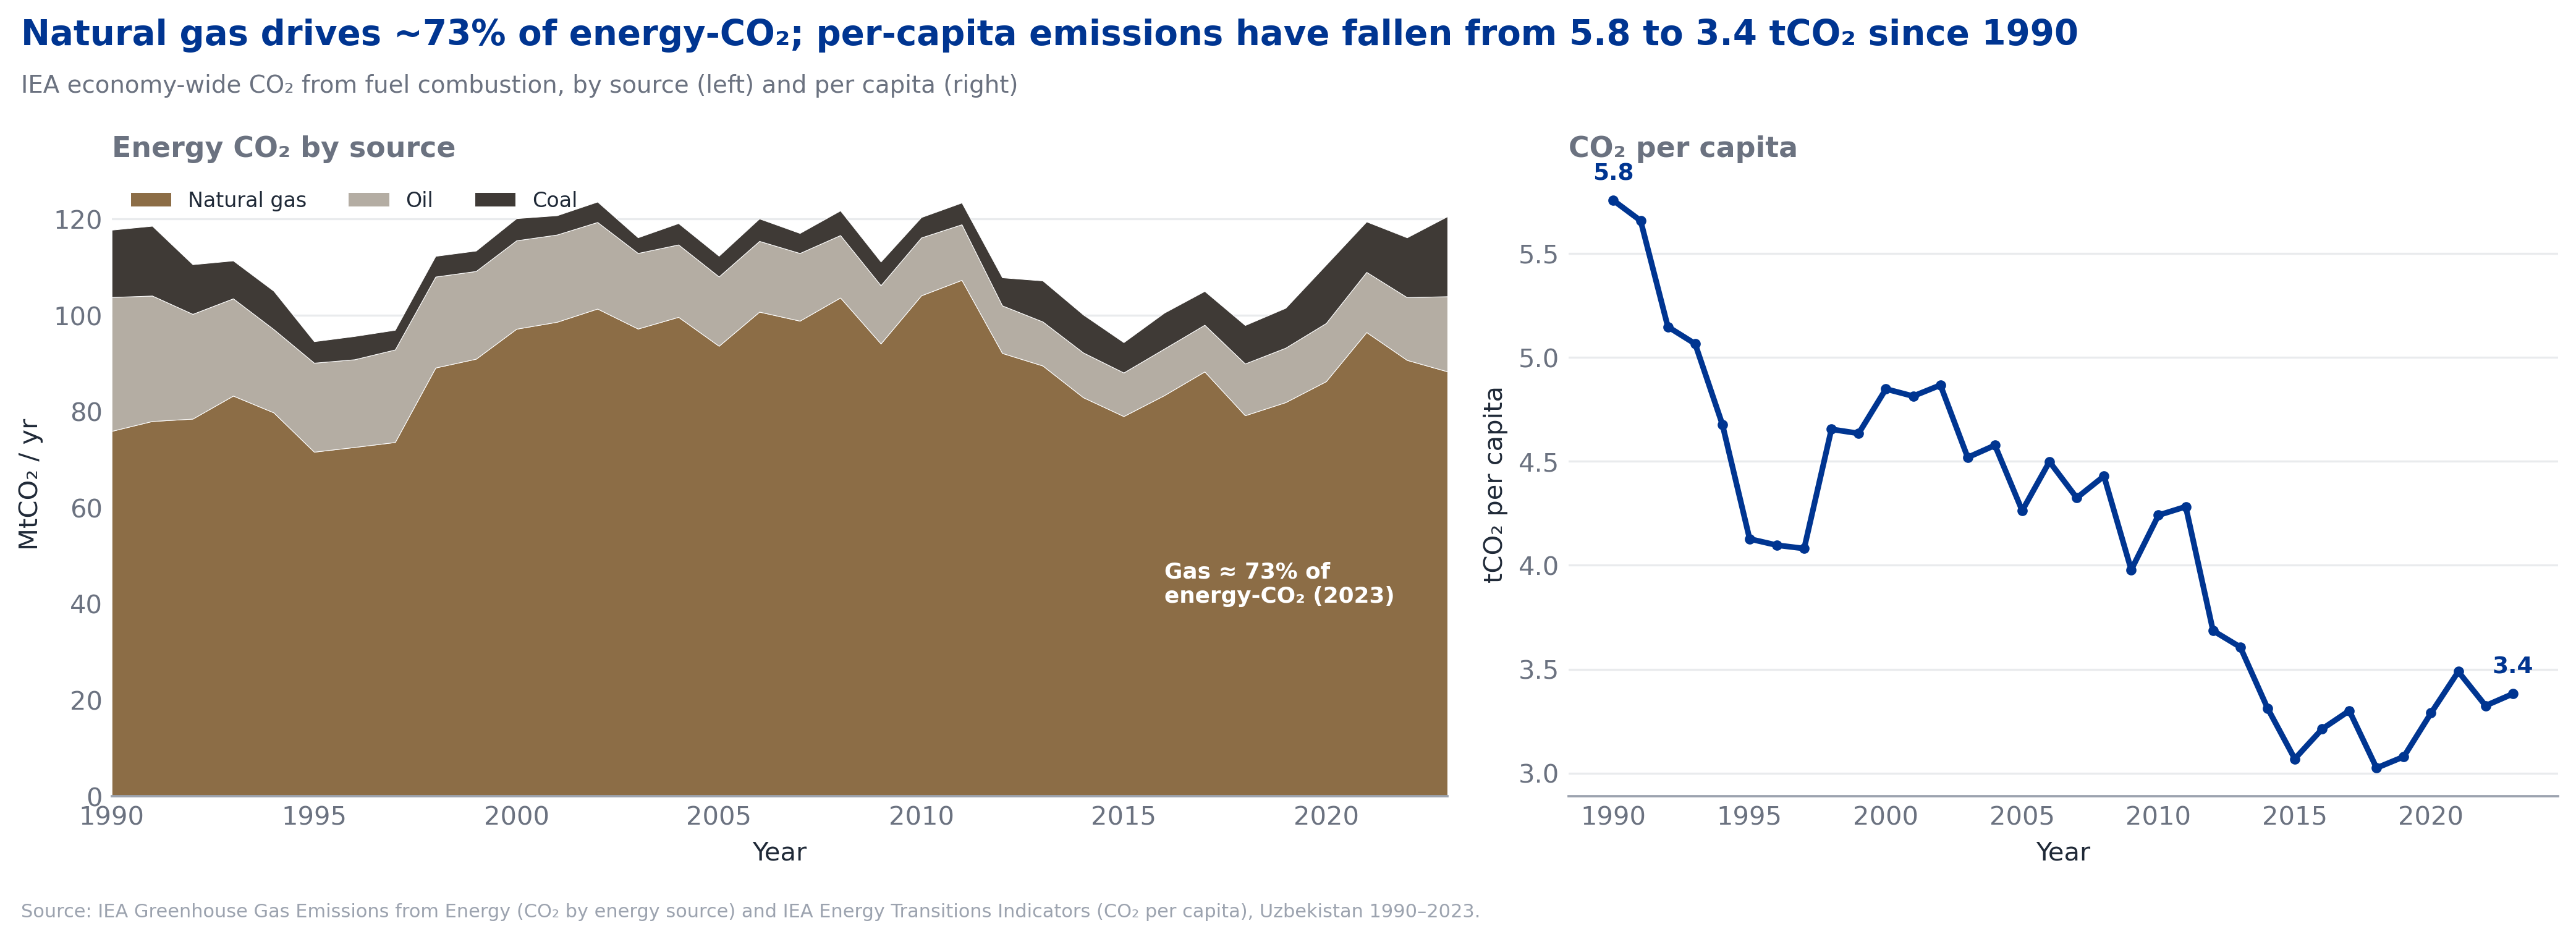
\includegraphics[width=\textwidth]{figures/appendixG_co2_economy.png}
\caption*{\itshape Figure G.1. Economy-wide CO\textsubscript{2} from fuel combustion by source (left, MtCO\textsubscript{2}) and per capita (right, tCO\textsubscript{2}), 1990--2023. Natural gas drives $\sim$73\% of combustion CO\textsubscript{2}; per-capita emissions fall from $\sim$5.8 to $\sim$3.4 tCO\textsubscript{2}. Source: IEA Greenhouse Gas Emissions from Energy and IEA Energy Transitions Indicators (IEA, 2024b).}
\end{figure*}

\textbf{Liquids: a shrinking, condensate-tilting pool.} Uzbekistan's liquid-fuels base has contracted sharply over the forecast-relevant period. Crude-oil output has fallen about \textbf{65\% since 2010}, and gas condensate is now the larger component of a shrinking total liquids pool --- a structural shift that leaves the refined slate (diesel, gasoline, fuel oil) dependent on a narrowing domestic feedstock (Figure G.2). This sits alongside the gas-balance signal of \S{}6.3: the same maturing upstream that pushes gas self-sufficiency below 100\% also thins the liquids supply, so the country's hydrocarbon base is narrowing on two fronts at once, reinforcing the strategic case for electrification and renewables.

\begin{figure*}[tp]
\centering
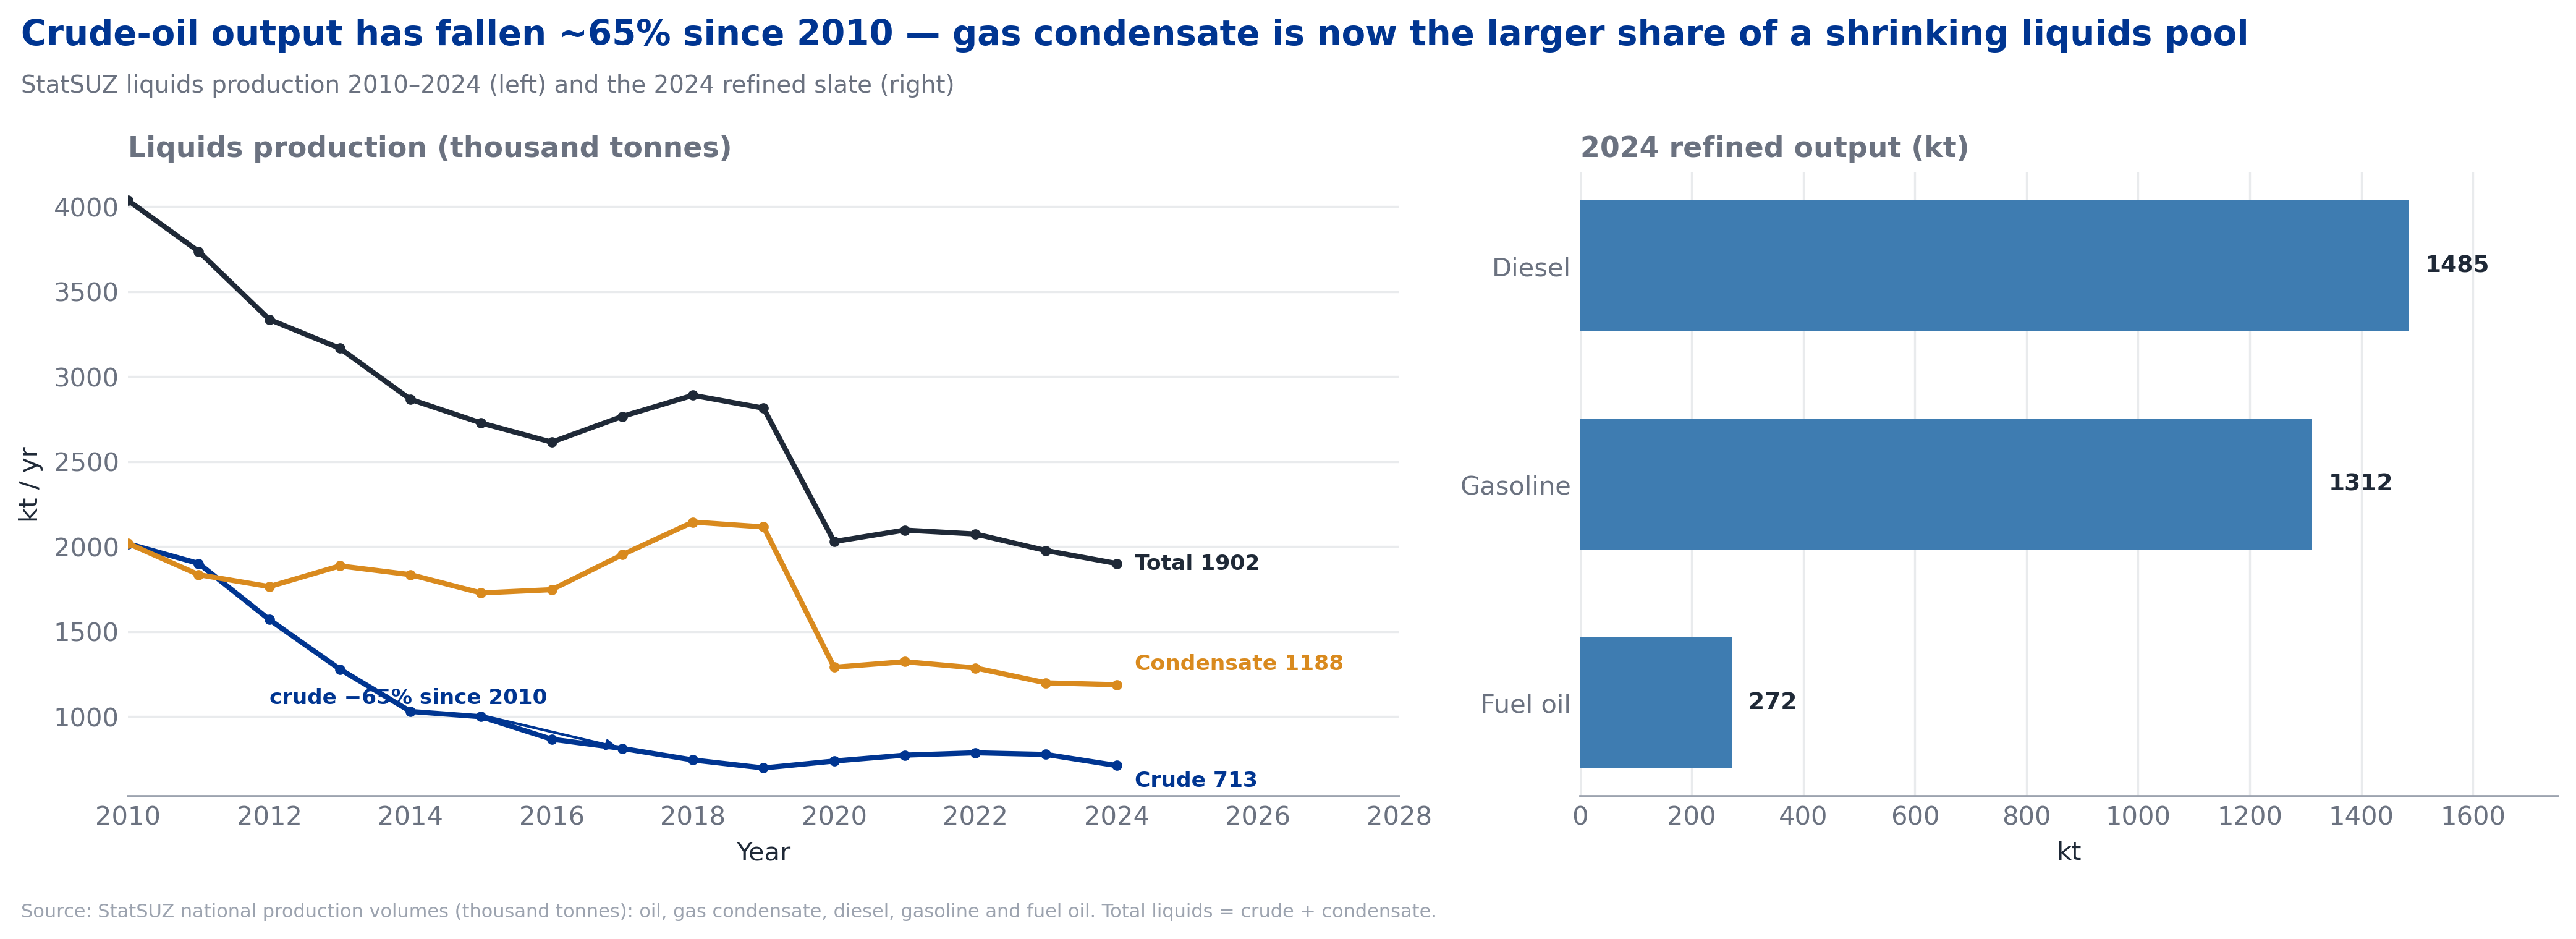
\includegraphics[width=\textwidth]{figures/appendixG_liquids.png}
\caption*{\itshape Figure G.2. Liquids production 2010--2024 (left, thousand tonnes: crude oil, gas condensate, and their total) and the 2024 refined slate (right, kt: diesel, gasoline, fuel oil). Crude output falls $\sim$65\% since 2010 as condensate becomes the larger share of a shrinking pool. Source: StatSUZ national production volumes (StatSUZ, 2024).}
\end{figure*}

\textbf{Primary energy supply: four-fifths gas.} At the level of total primary energy supply, Uzbekistan is among the most gas-concentrated systems in the world: natural gas supplies roughly \textbf{79\% of primary energy}, with oil and coal making up most of the rest and non-hydro renewables still a sliver even at the end of the record (Figure G.3). This is the structural fact behind every decarbonisation lever in the report --- a system this gas-bound cannot decarbonise by re-dispatch, only by building alternative supply, which is precisely why the transition reads throughout as a construction story rather than an operational one.

\begin{figure*}[tp]
\centering
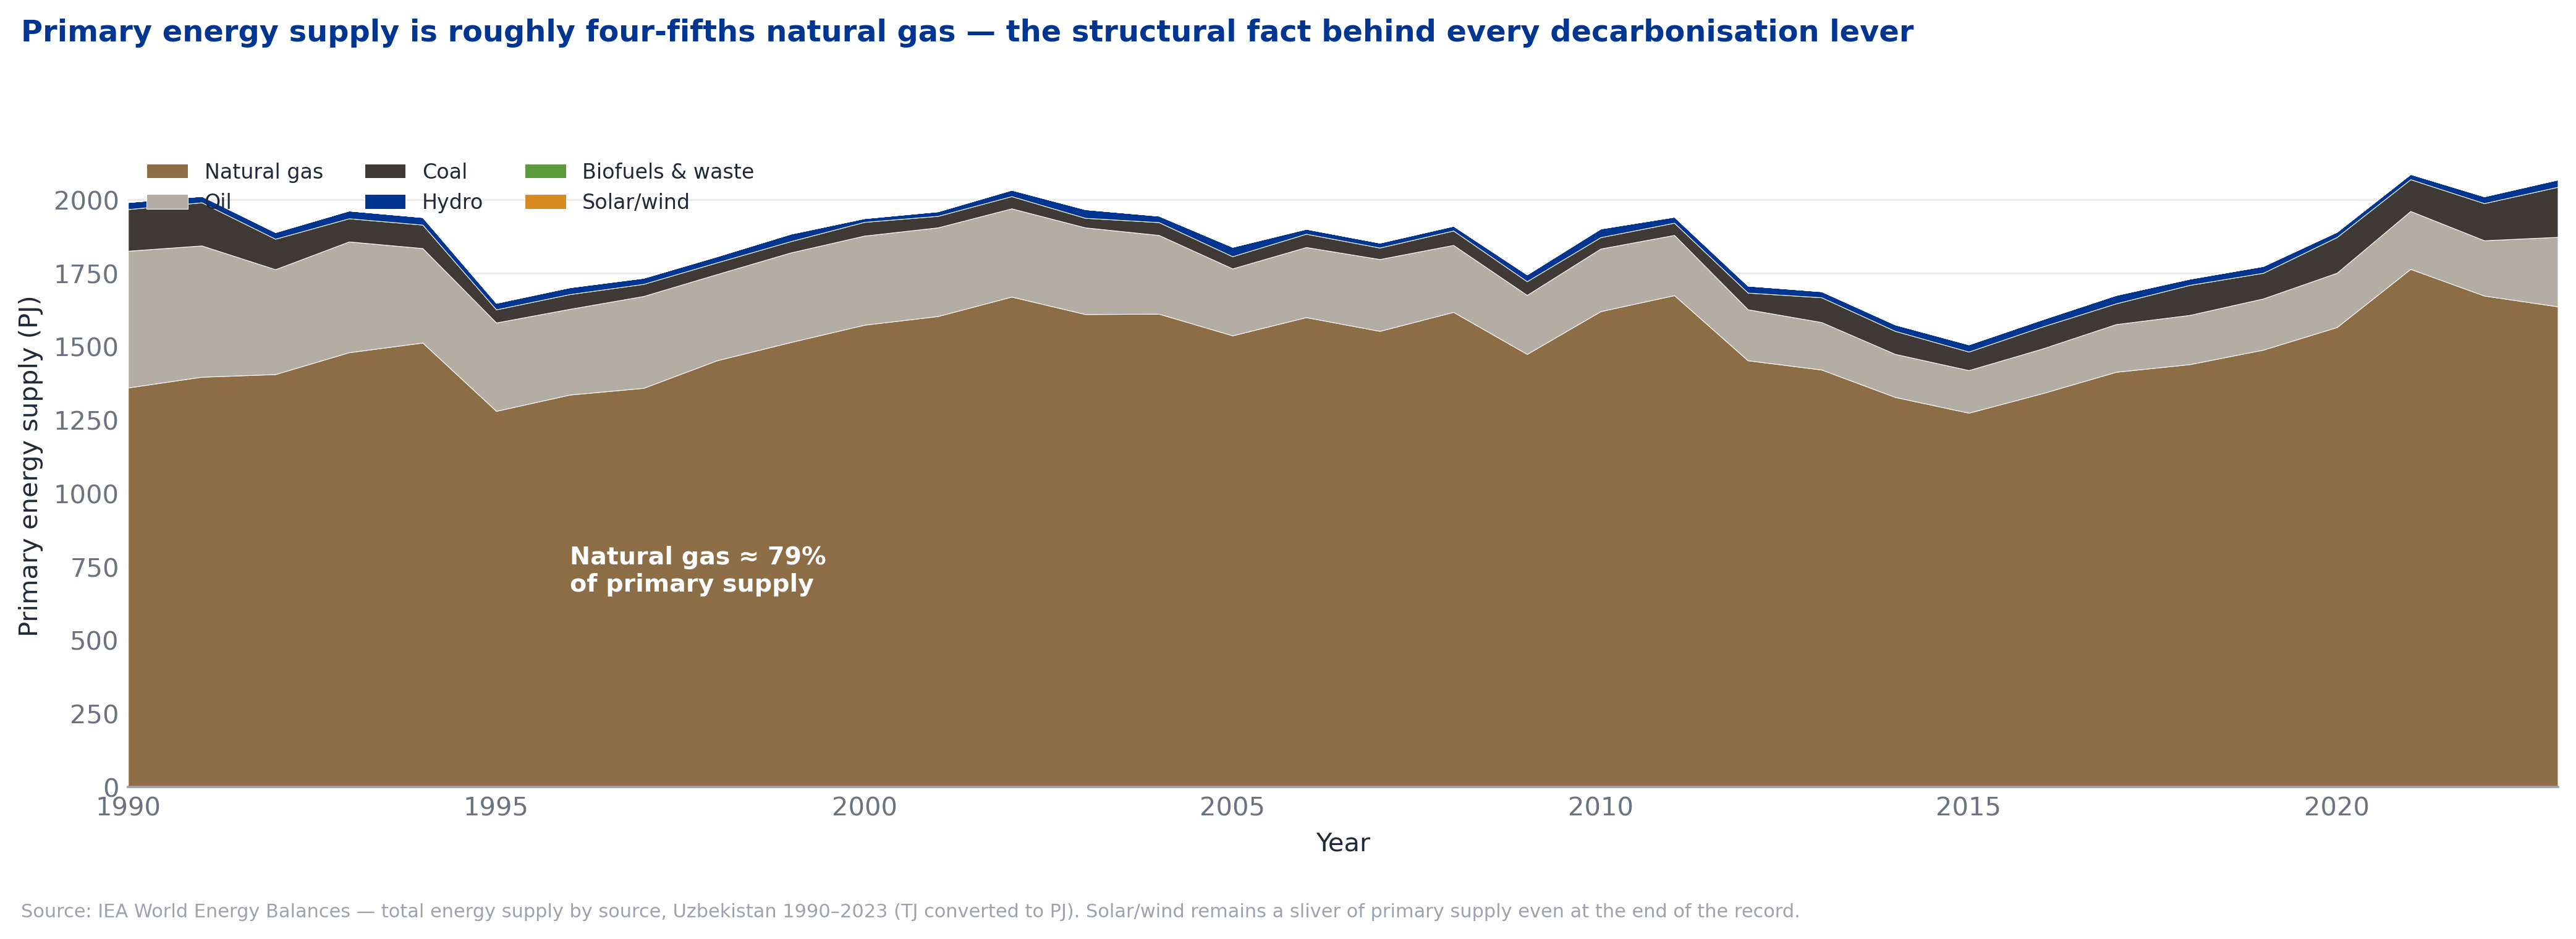
\includegraphics[width=\textwidth]{figures/appendixG_primary_energy.png}
\caption*{\itshape Figure G.3. Total primary energy supply by source, 1990--2023 (PJ): natural gas, oil, coal, hydro, biofuels \& waste, and solar/wind. Natural gas is $\sim$79\% of primary supply throughout; solar and wind remain a sliver even at the end of the record. Source: IEA World Energy Balances (IEA, 2024e).}
\end{figure*}

\begin{figure*}[tp]
\centering
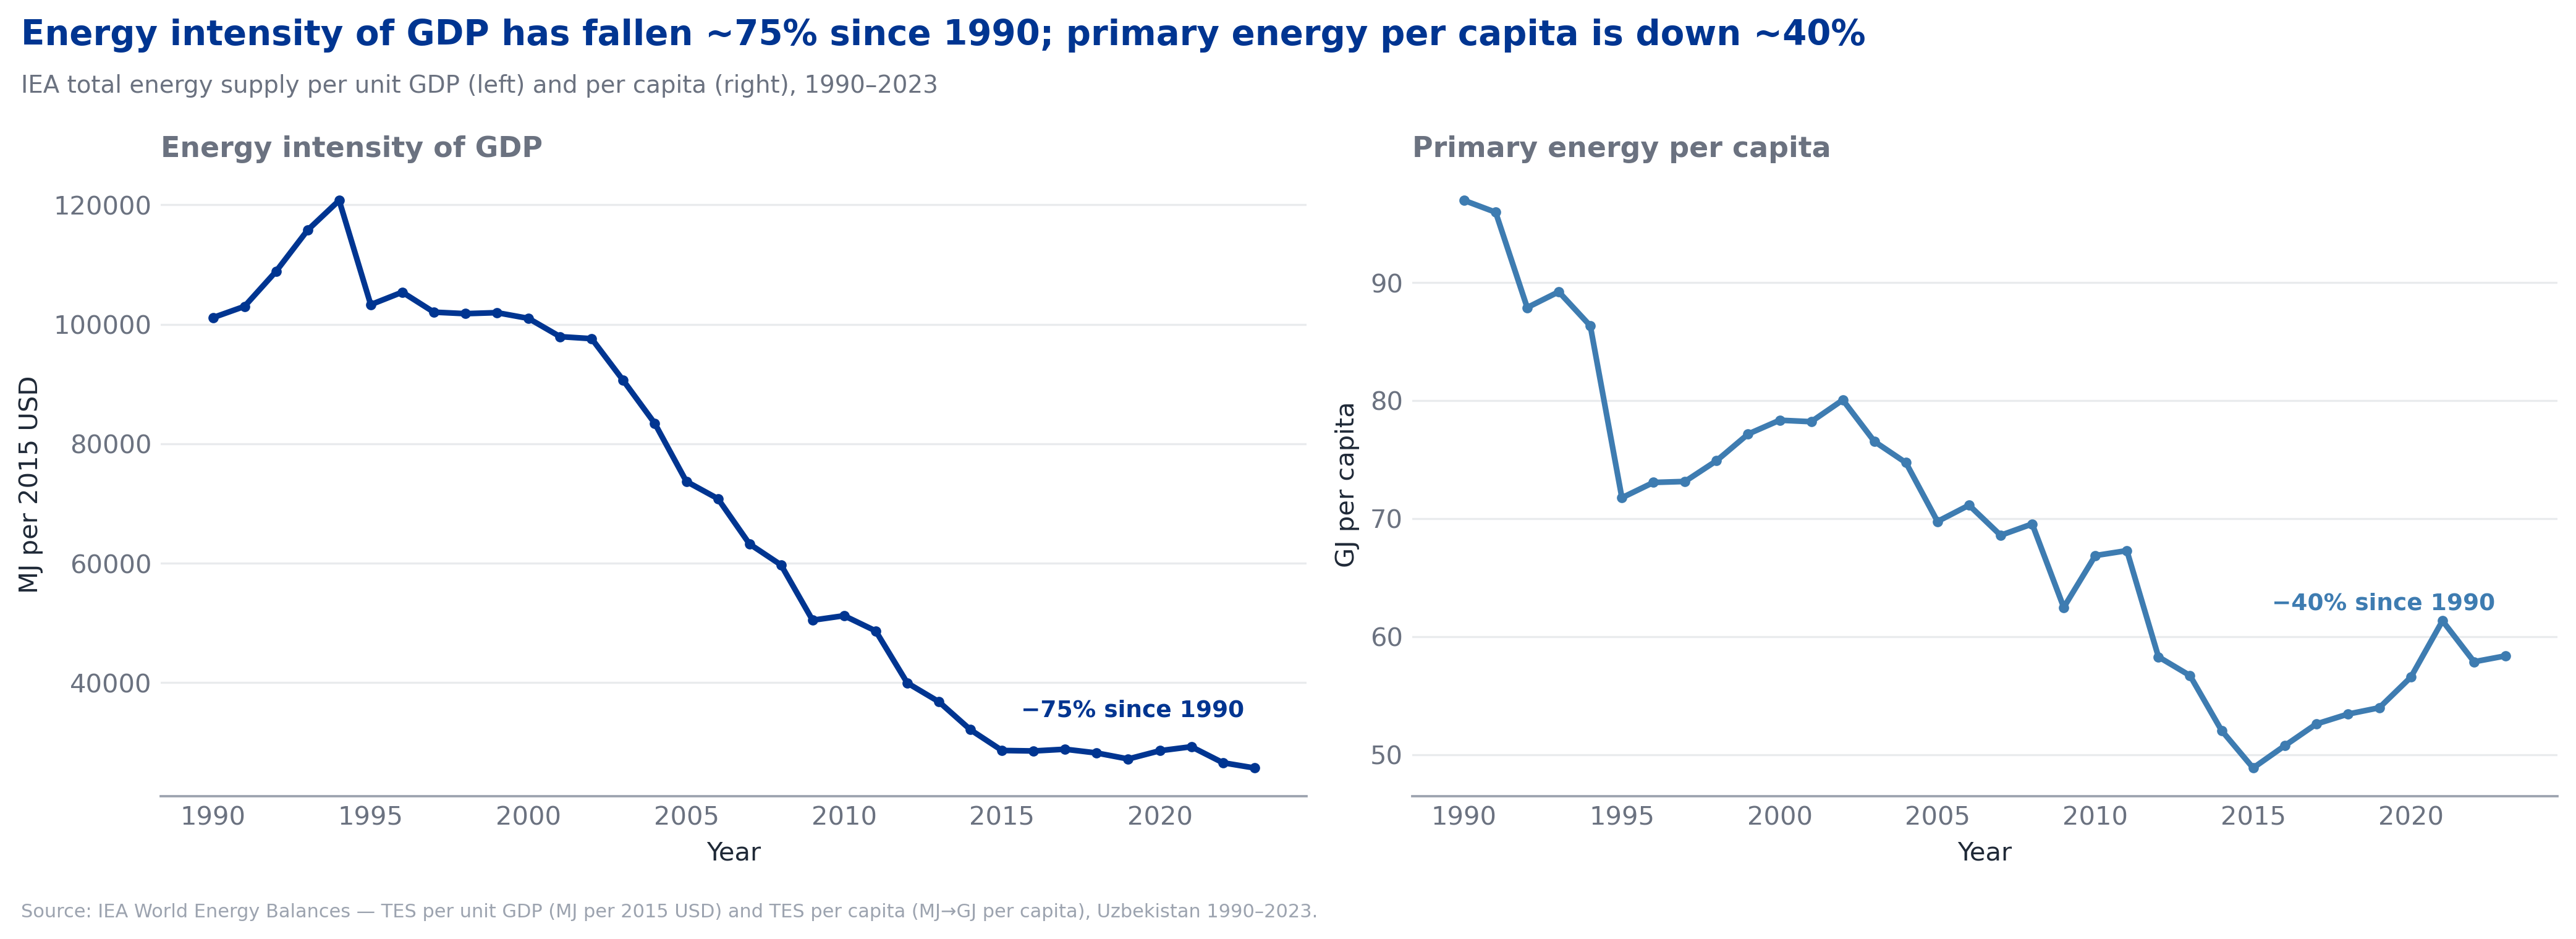
\includegraphics[width=\textwidth]{figures/appendixG_energy_intensity.png}
\caption*{\itshape Figure G.4. Energy intensity of GDP (left, MJ per 2015 USD) and primary energy per capita (right, GJ per capita), 1990--2023. Intensity falls $\sim$75\% and per-capita supply $\sim$40\% as the post-Soviet economy de-intensifies. The intensity level is large because it is measured against market-exchange-rate USD GDP, as reported by the IEA; the decline is the salient feature. Source: IEA World Energy Balances (IEA, 2024e).}
\end{figure*}

\textbf{Energy intensity: a steep, sustained de-intensification.} The one unambiguously favourable long-run trend is efficiency. Energy intensity of GDP has fallen about \textbf{75\% since 1990}, and primary energy per capita is down about \textbf{40\%} over the same window (Figure G.4) --- the economy now extracts far more output from each unit of energy than the late-Soviet system did. This de-intensification is what allows the per-capita emissions decline of G.1 to coexist with sustained economic growth, and it is the macro backdrop against which the report's $\sim$9\% forward grid-loss target (\S{}6.1) is plausible: the system has demonstrated, at the economy-wide level, that large efficiency gains are achievable, even as the grid-loss component of that efficiency story remains stubbornly unrealised.

\textbf{The four exhibits, read as one.} Taken together, the four panels describe a single energy system caught between a heavy structural inheritance and a genuine, decades-long efficiency gain, and they explain why the report treats Uzbekistan's transition as a construction problem rather than a dispatch problem. The inheritance is gas: roughly four-fifths of primary energy (G.3) and about three-quarters of economy-wide combustion CO\textsubscript{2} (G.1) trace to a single fuel, a concentration no amount of re-dispatch can unwind, because no idle low-carbon capacity waits behind the gas fleet. The upstream that supplies that gas is itself maturing --- crude output down about \textbf{65\% since 2010}, condensate now the larger share of a shrinking liquids pool (G.2) --- so the hydrocarbon base is narrowing on two fronts at once even as electricity demand is set to rise. Against that backdrop the efficiency record (G.4) is the one unambiguously favourable trend, and it carries a specific analytical weight: an economy that has already taken roughly three-quarters out of its energy intensity since 1990 has demonstrated, at the macro scale, that the order of efficiency gain the report's grid-loss target assumes is achievable in practice, not merely in principle. The unrealised piece is narrower --- the network-loss component specifically, a well-bounded target inside a system that has already proven it can de-intensify. That is the precise sense in which this appendix reinforces the main argument: the demand the model projects, the supply gap the scenarios open, and the loss reduction the investment signals price are all expressions of one structural fact --- a gas-bound but intensity-improving system whose decarbonisation must be built rather than dispatched, and whose most credible near-term efficiency win is the grid itself.

\end{document}